\documentclass[9pt,twocolumn,twoside]{gsajnl_modified}
% Use the documentclass option 'lineno' to view line numbers

\usepackage[htt]{hyphenat}  % https://tex.stackexchange.com/a/543
\usepackage[export]{adjustbox}

\PassOptionsToPackage{hyphens}{url}\usepackage{hyperref}
\hypersetup{draft}  % comment out hyperlinks for now to deal with line-breaking issue in references

\articletype{inv} 

\title{Recovery of a deleted deep sequencing data set sheds more light on the early Wuhan SARS-CoV-2 epidemic}

\author[]{\Large Jesse D. Bloom}

\affil[]{Fred Hutchinson Cancer Research Center}
\affil[]{Howard Hughes Medical Institute}
\affil[]{Seattle, WA, USA}

\keywords{}

\runningtitle{} % For use in the footer 
\runningauthor{}

\begin{abstract}
Abstract here
\end{abstract}

\begin{document}

\maketitle
\thispagestyle{firststyle}
%\marginmark
\firstpagefootnote

\correspondingauthoraffiliation{}{Corresponding author: \href{mailto:jbloom@fredhutch.org}{jbloom@fredhutch.org}}
\vspace{-33pt}% Only used for adjusting extra space in the left column of the first page

\lettrine[lines=2]{\color{color2}T}{}he origins... 

\section{Results}

\subsection{Identification of a SARS-CoV-2 deep sequencing data set that has been removed from the NCBI's Sequence Read Archive}
During the course of my research, I read a paper by \citet{farkas2020insights} that analyzed SARS-CoV-2 deep sequencing data from the Sequence Read Archive (SRA), which is a repository maintained by the NIH's National Center for Biotechnology Information (NCBI).
The first supplementary table of \citet{farkas2020insights} lists all SARS-CoV-2 deep sequencing data available from the SRA as of March 30, 2020.

The majority of entries in this table refer to a project (BioProject PRJNA612766) by Wuhan University that is described as nanopore sequencing of SARS-CoV-2 amplicons.
The table indicates this project represents 241 of the 282 SARS-CoV-2 sequencing run accessions in the SRA as of March, 30, 2020.
Because I had never encountered any other mention of this project, I performed a Google search for ``PRJNA612766,'' and found no search hits other than the supplementary table itself.
Searching for ``PRJNA612766'' in the NCBI's SRA search box returned a message of ``No items found.''
I then searched for individual sequencing run accessions from the project in the NCBI's SRA search box.
These searches returned messages indicating that the sequencing runs had been removed (Figure~\ref{fig:acc_removed}).

\begin{figure}[]
\centering
\fbox{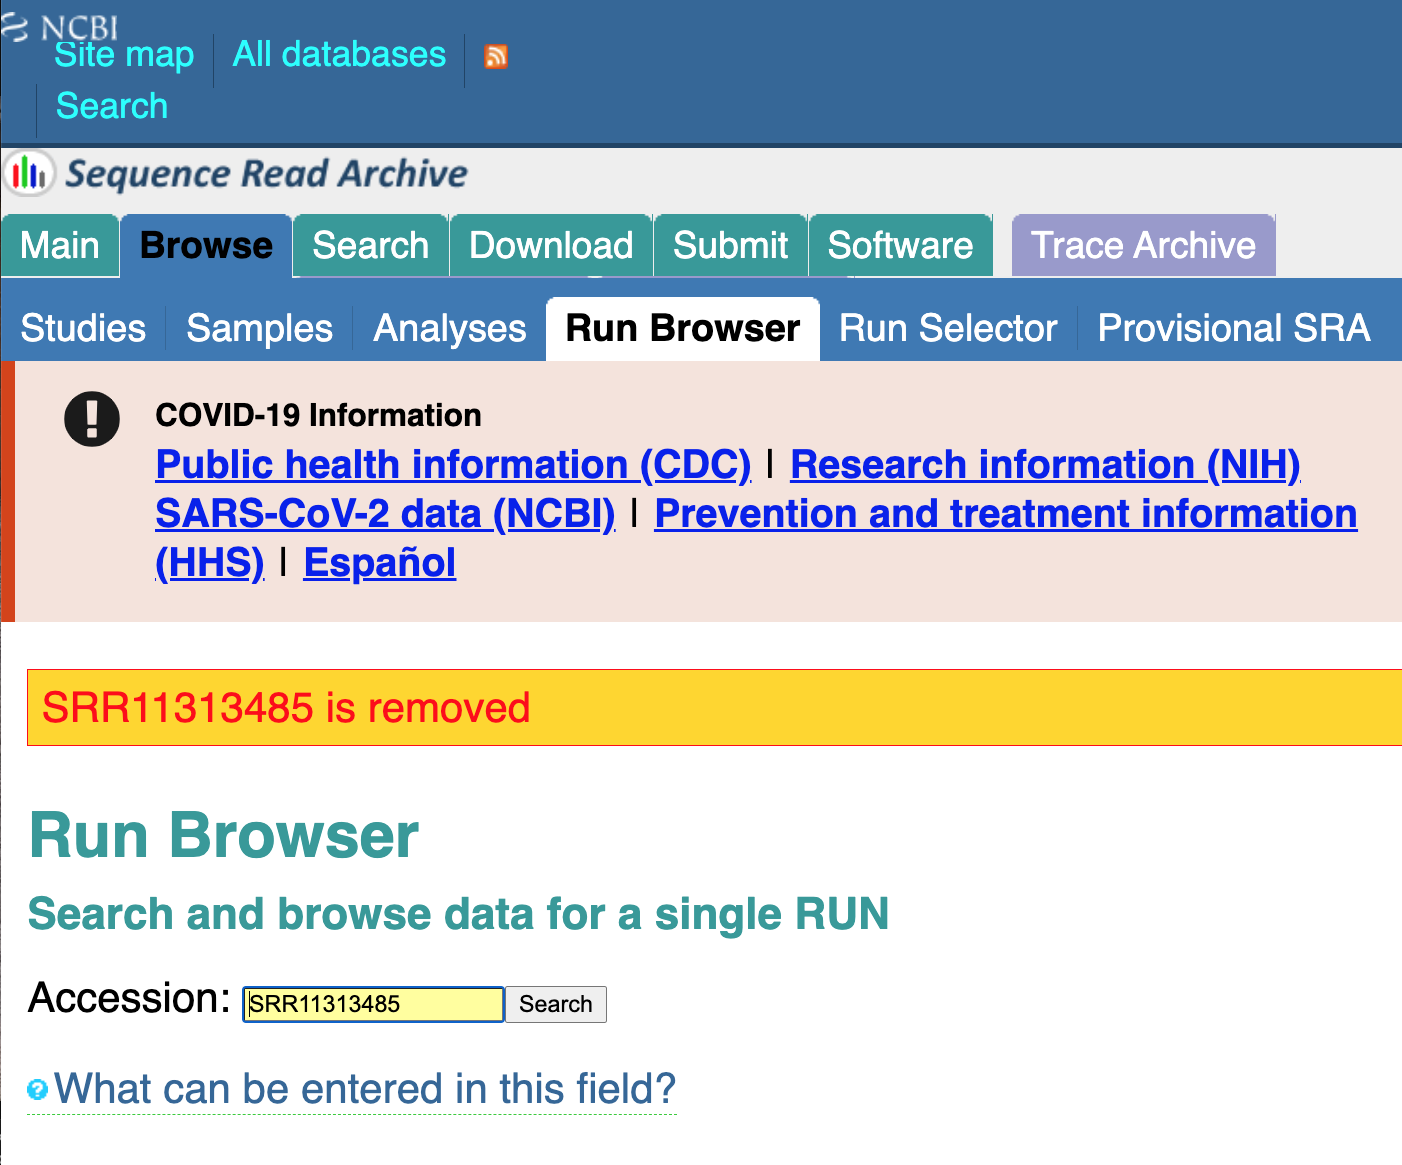
\includegraphics[trim={0.2in 0 0 9in},clip,width=\linewidth]{figures/acc_removed.png}}
\caption{Accessions from deep sequencing project PRJNA612766 have been removed from the SRA.
Shown is the result of searching for ``SRR11313485'' in the SRA search toolbar.
This result has been digitally archived on the Wayback Machine at \url{https://web.archive.org/web/20210502131630/https://trace.ncbi.nlm.nih.gov/Traces/sra/?run=SRR11313485}.
}%
\label{fig:acc_removed}
\end{figure}

The SRA is designed as a permanent archive of deep sequencing data.
The SRA documentation states that after a sequencing run is uploaded, ``neither its files can be replaced nor filenames can be changed,'' and that data can only be deleted by e-mailing SRA staff~\citep{SRA_deletion}.
An example of this process from another study is in Figure~\ref{fig:pangolin_emails}, which shows an e-mail sent to SRA staff by the lead author of a paper on pangolin coronaviruses~\citep{xiao2020isolation} to request the deletion of two sequencing runs.
Subsequent to March 30, 2020, a similar e-mail request must have been made to fully delete SARS-CoV-2 deep sequencing project PRJNA612766.

\begin{figure}[]
\centering
\fbox{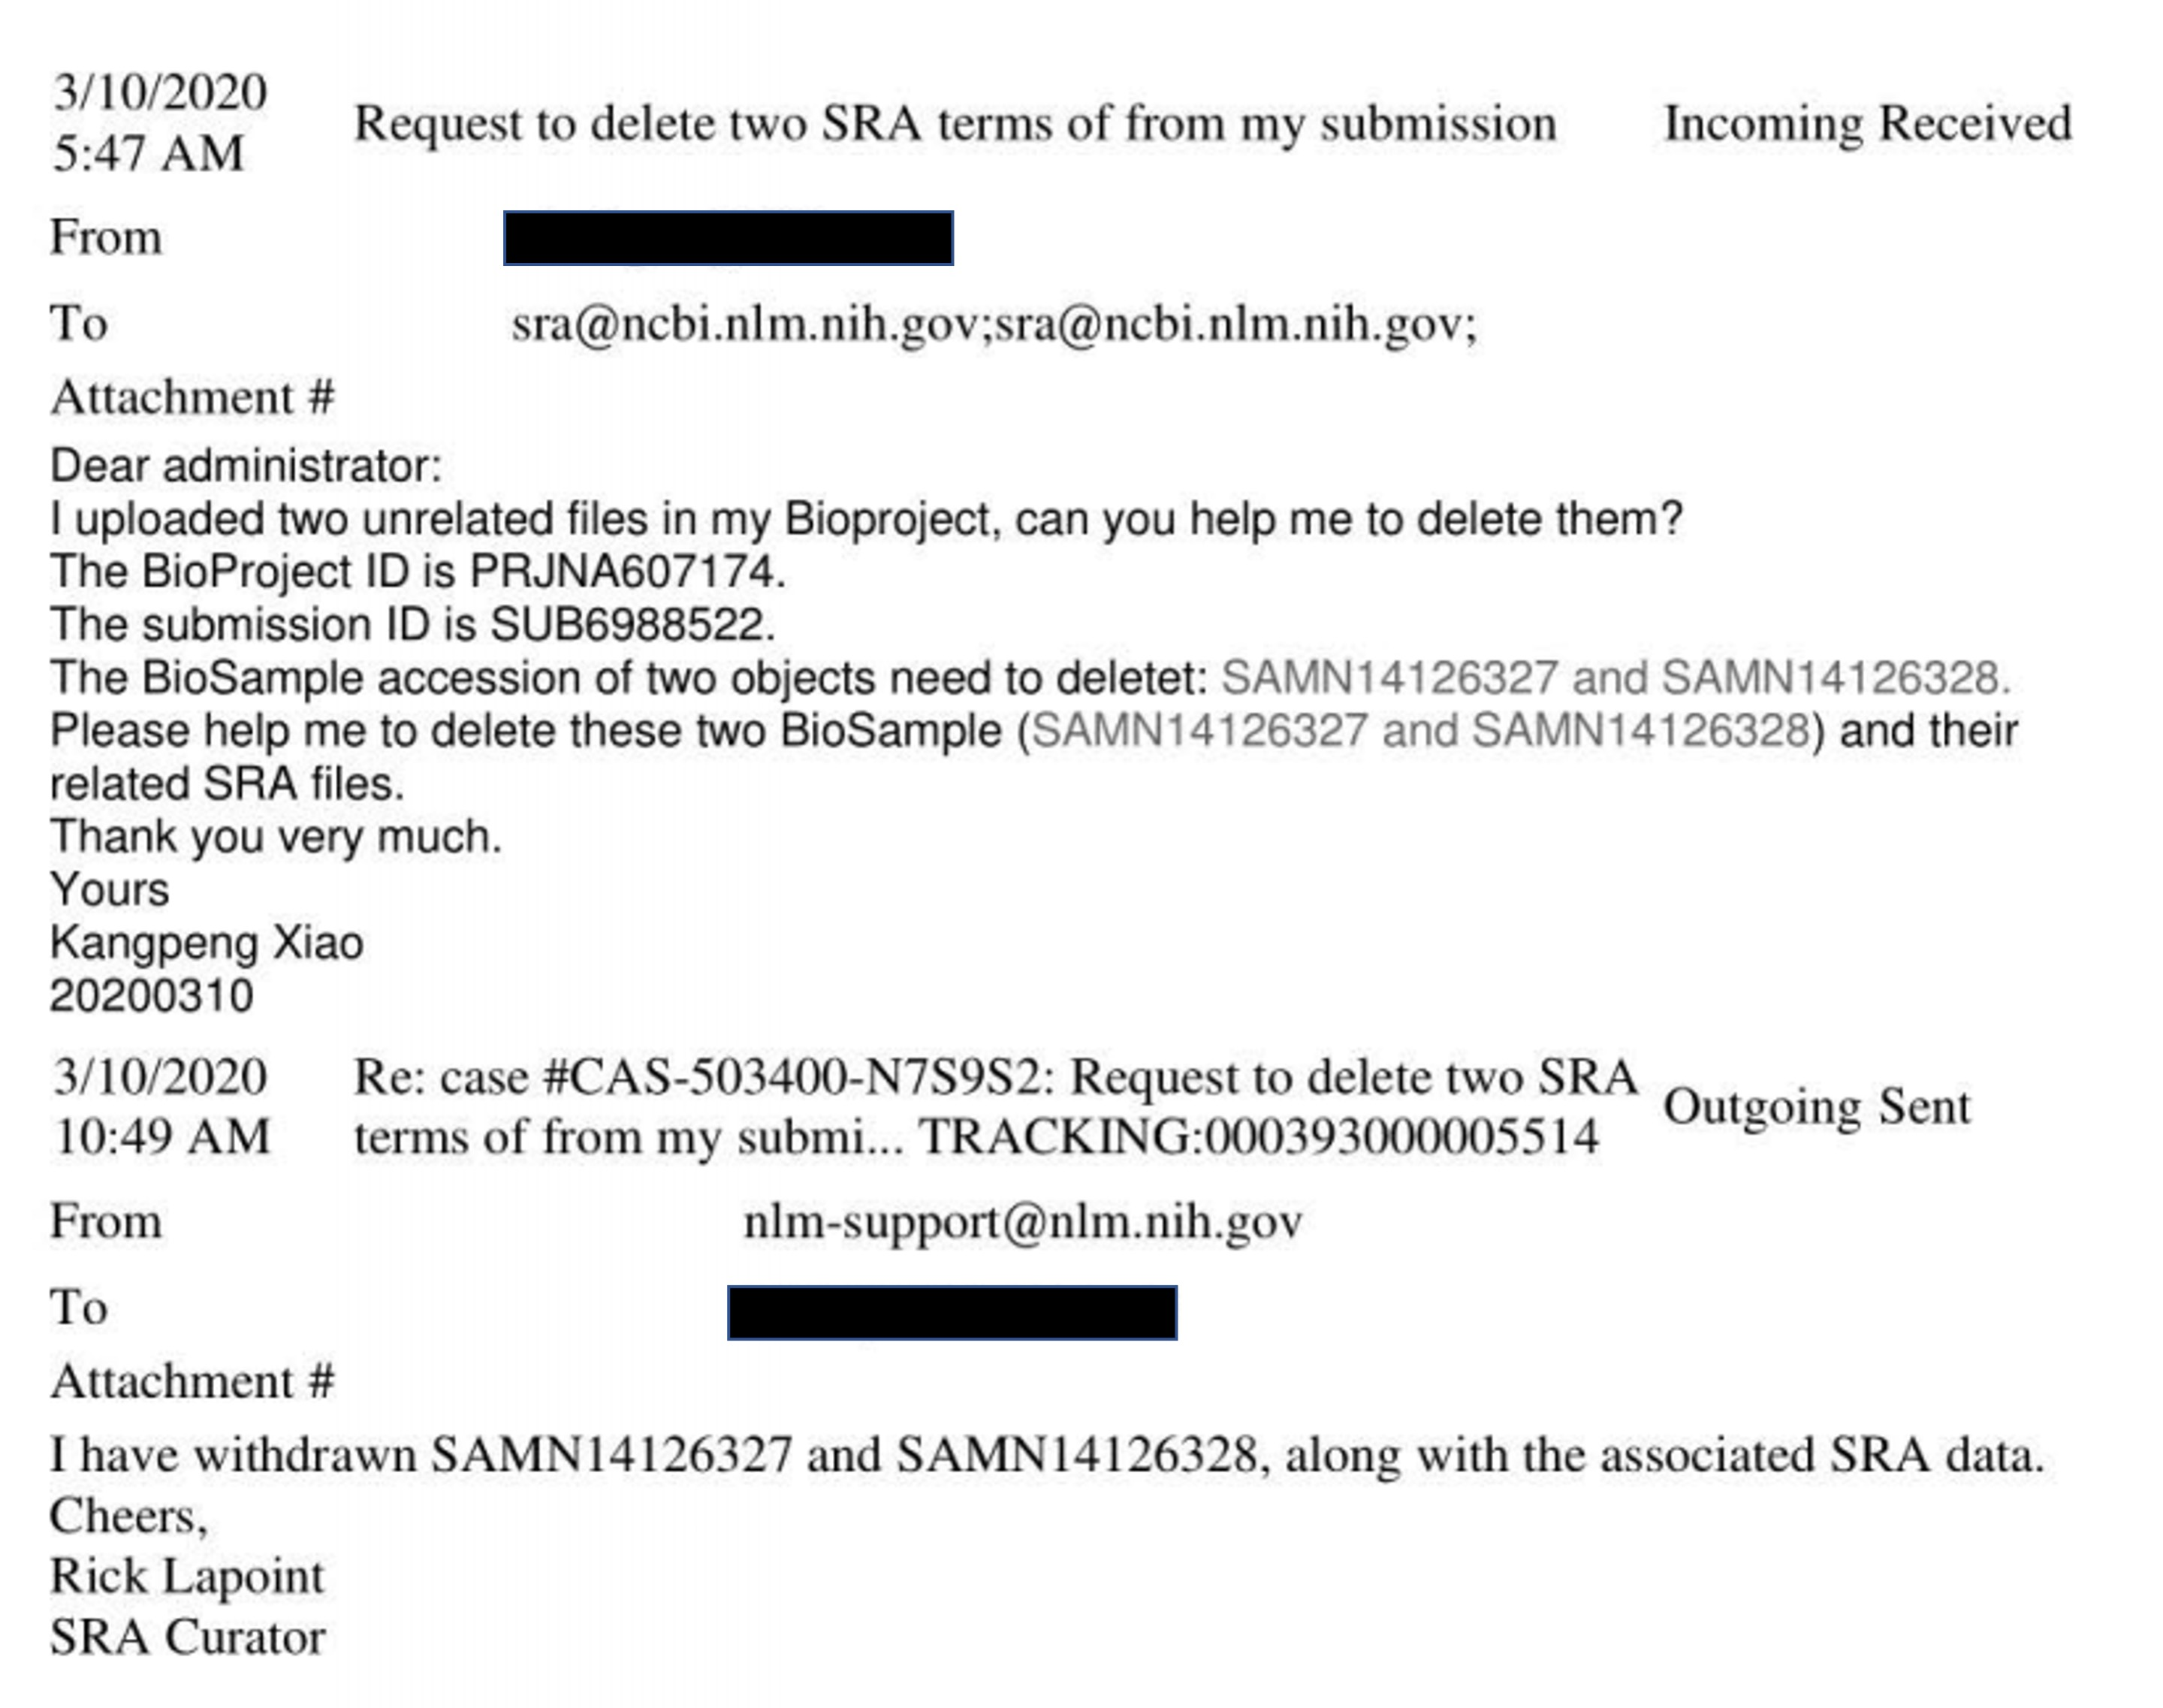
\includegraphics[trim={0.8in 0.8in 1.1in 1in},clip,width=\linewidth]{figures/pangolin_emails.jpg}}
\caption{Example of the process to delete SRA data.
The image shows excerpted e-mails between the lead author of the pangolin coronavirus paper~\citet{xiao2020isolation} and SRA staff.
The full e-mails are at \url{https://usrtk.org/tag/pangolin-papers/}.
}
\label{fig:pangolin_emails}
\end{figure}

\subsection{The deleted data set contains sequencing of viral samples collected early in the Wuhan epidemic}
The metadata in the first supplementary table of \citet{farkas2020insights} indicates that the samples in deleted project PRNJA612766 were collected by Aisu Fu and Renmin Hospital of Wuhan University.
Google searching for these terms revealed the samples were related to a study posted as a pre-print on \textit{medRxiv} in early March of 2020~\citep{wang2020medRxiv}, and subsequently published in the journal \textit{Small} in June of 2020~\citep{wang2020small}.

The study describes an approach to diagnose infection with SARS-CoV-2 and other respiratory viruses by nanopore sequencing.
This approach involved reverse-transcription of total RNA from swab samples, followed by PCR with specific primers to generate amplicons covering portions of the viral genome.
These amplicons were then sequenced on an Oxford Nanopore GridION, and infection was diagnosed if the sequencing yielded sufficient reads aligning to the viral genome.
Importantly, the study notes that this approach yields information about the sequence of the virus as well enabling diagnosis of infection.

The pre-print~\citep{wang2020medRxiv} says the approach was applied to ``45 nasopharyngeal swab samples from outpatients with suspected COVID-19 early in the epidemic.''
The digital object identifier (DOI) for the pre-print indicates that it was processed by \textit{medRxiv} on March 4, 2020, which is one day after China's State Council ordered that all papers related to COVID-19 must be approved by a centralized group to ensure that scientific publications were coordinated ``like moves in a game of chess''~\citep{Kang2020}.
The final published manuscript~\citep{wang2020small} from June of 2020 updated the description from ``early in the epidemic'' to ``early in the epidemic (January 2020).''
Both the pre-print and published manuscript say that 34 of the 45 early epidemic samples were positive in the sequencing-based diagnostic approach.
In addition, both state that the approach was later applied to 16 additional samples collected on February 11--12, 2020, from SARS-CoV-2 patients hospitalized at Renmin Hospital of Wuhan University.

There is complete concordance between the accessions for project PRJNA612766 in the supplementary table of \citet{farkas2020insights} and the samples described by \citet{wang2020medRxiv}.
There are 89 accessions corresponding to the 45 early epidemic samples, with these samples named like wells in a 96-well plate (A1, A2, etc).
The number of accessions is approximately twice the number of early epidemic samples because each sample has data for two sequencing runtimes except one sample (B5) with just one runtime.
 There are 31 accessions corresponding to the 16 samples collected in February from Renmin Hospital patients, with these samples named R01, R02, etc.
 Again, all but one sample (R04) have data for two sequencing runtimes.
 In addition, there are 7 accessions corresponding to positive and negative controls, 2 accessions corresponding to other respiratory virus samples, and 112 samples corresponding to plasmids used for benchmarking of the approach.
 Together, these samples and controls account for all 241 accessions listed for PRJNA612766 in the supplementary table of \citet{farkas2020insights}.

Neither the pre-print~\citep{wang2020medRxiv} nor published manuscript~\citep{wang2020small} contain any correction or note that indicates a scientific reason for deleting the study's sequencing data from the SRA.
I e-mailed both corresponding authors of \citet{wang2020medRxiv} to ask why they had deleted the deep sequencing data and to request details on the collection dates of the early outpatient samples, but received no reply.

\subsection{Recovery of deleted sequencing data from the Google cloud} 
As indicated in Figure~\ref{fig:acc_removed}, none of the deleted sequencing runs could be accessed through the SRA's web interface.
In addition, none of the runs could be accessed using the command-line tools of the SRA Toolkit.
For instance, as of June 3, 2020, running \texttt{fastq-dump SRR11313485} or \texttt{vdb-dump SRR11313485} returned an error message stating ``err: query unauthorized while resolving query within virtual file system module - failed to resolve accession 'SRR11313485'``.

However, the SRA has begun storing all data on the Google and Amazon clouds.
While inspecting the SRA's web interface for other sequencing accessions, I noticed that SRA files are often available from links to the cloud such as \texttt{https://storage.googleapis.com/nih-sequence-read-archive/run/<ACCESSION>/<ACCESSION>}.

Based on the hypothesis that deletion of sequencing runs by the SRA might not remove files stored on the cloud, I interpolated the cloud URLs for the deleted accessions and tested if they still yielded the SRA files.
This strategy was successful; for instance, as of June 3, 2020, going to \url{https://storage.googleapis.com/nih-sequence-read-archive/run/SRR11313485/SRR11313485} downloads the SRA file for accession SRR11313485.
I have archived this file on the Wayback Machine at \url{https://web.archive.org/web/20210502130820/https://storage.googleapis.com/nih-sequence-read-archive/run/SRR11313485/SRR11313485}.

I automated this strategy to download the SRA files for 97 of the 99 sequencing runs corresponding to the 34 SARS-CoV-2 positive early epidemic samples and the 16 hospital samples from February (files for SRR11313490 and SRR11313499 were not accessible via the cloud).
I used the SRA Toolkit to get the object timestamp (\texttt{vdb-dump -{}-obj\_timestamp}) and time (\texttt{vdb-dump -{}-info}) for each SRA file.
For all files, the object timestamp is February 15, 2020, and the time is March 16, 2020.
Although the SRA Toolkit does not clearly document these two properties, my \emph{guess} is that the object timestamp may refer to when the SRA file was created from a FASTQ file uploaded to the SRA, and the time may refer to when the accession was made public.

\subsection{The data are sufficient to determine the viral sequence from the start of spike through the end of ORF10 for some samples}
The approach of \citet{wang2020medRxiv} involved sequencing PCR amplicons covering nucleotide sites 21,563 to 29,674 of the SARS-CoV-2 genome, which spans from the start of the spike gene to the end of ORF10.
The approach also involved sequencing a short amplicon generated by nested PCR that covered a fragment of ORF1ab spanning sites $\sim$15,080 to 15,550.
In this paper, I only analyze the region from spike through ORF10 because this is a much longer contiguous sequence and the amplicons were generated by a single rather than nested PCR.
I slightly trimmed the region of interest to sites 21,570 to 29,550 because many samples had poor coverage at the termini of the region.

I aligned the recovered deep sequencing data to the SARS-CoV-2 genome using \texttt{minimap2}~\citep{li2018minimap2}, combining accessions for the same sample.
Figure~\ref{suppfig:coverage} shows the sequencing coverage for the 34 virus-positive early epidemic samples and the 16 hospitalized patient samples over the region of interest; a comparable plot for the whole genome is in Figure~\ref{suppfig:coverage_all}.

\begin{table*}[]
{\small
\begin{tabular}{lrll}
\toprule
sample &  fraction sites called (21570-29550) &           patient group &                                        substitutions relative to proCoV2 \\
\midrule
A4 &                               0.9827 &        early outpatient &                                                                          none \\
C1 &                               0.9966 &        early outpatient &  G22081A (A=924, C=4, G=9), C28144T (C=6, T=1185), T29483G (C=1, G=45, T=1) \\
C2 &                               0.9962 &        early outpatient &                                                 C29095T (C=1, G=1, T=751)  \\
C9 &                               0.9536 &        early outpatient &                                  C28144T (C=3, T=823), G28514T (G=1, T=36)  \\
D9 &                               0.9585 &        early outpatient &                                                     C28144T (C=4, T=1653)  \\
D12 &                               0.9970 &        early outpatient &                                                     C28144T (C=8, T=2400)  \\
E1 &                               0.9759 &        early outpatient &                                                           C28144T (T=125)  \\
E5 &                               0.9758 &        early outpatient &              C24034T (A=5, C=3, T=74), T26729C (C=12), G28077C (C=142, G=4)  \\
E11 &                               0.9877 &        early outpatient &                                 C25460T (C=2, T=246), C28144T (C=1, T=412)  \\
F11 &                               0.9594 &        early outpatient &                             T25304A (A=9, T=1), C28144T (C=6, G=1, T=1328)  \\
G1 &                               0.9959 &        early outpatient &                                   none                                        \\
G11 &                               0.9677 &        early outpatient &                                  none                                         \\
H9 &                               0.9941 &        early outpatient &                                                     C28144T (C=2, T=1254)  \\
R11 &                               0.9987 &  hospital patient (Feb) &                               C21707T (T=401), C28144T (A=1, C=18, T=4265)  \\
\bottomrule
\end{tabular}
}
\caption{Samples for which the SARS-CoV-2 sequence could be called at $\ge$95\% of sites between 21,570 and 29,550, and the substitutions in this region relative to the putative SARS-CoV-2 progenitor proCoV2 inferred by \citet{kumar2021evolutionary}.
Numbers in parentheses after each substitution give the deep sequencing reads with each nucleotide identity.
\label{tab:mutations}
}
\end{table*}

I called the consensus viral sequence for each sample at each site with coverage $\ge$3 and $>$80\% of the reads concurring on the nucleotide identity.
With these criteria, 13 of the early outpatient samples and 1 of the February hospitalized patient samples had sufficient coverage to call the consensus sequence at $>$95\% of the sites in the region of interest (Table~\ref{tab:mutations}), and for the remainder of this paper I focus on these high-coverage samples.
Table~\ref{tab:mutations} also shows the mutations in each sample relative to proCoV2, which is a putative progenitor of SARS-CoV-2 inferred by \citet{kumar2021evolutionary} that differs from the widely using Wuhan-Hu-1 reference sequence by three mutations (C8782T, C18060T, and T28144C).
Although requiring coverage of only $\ge$3 is relatively lenient, Table~\ref{tab:mutations} shows that all sites with mutations have coverage $\ge$10.
In addition, the mutations I called from the raw sequence data in Table~\ref{tab:mutations} concord with those mentioned in \citet{wang2020small}.

I also determined the consensus sequence of the plasmid control used by \citet{wang2020medRxiv} from the recovered sequencing data, and found that it had mutations C28144T and G28085T relative to proCoV2, which means that in the region of interest this control matches Wuhan-Hu-1 with the addition of G28085T.
Since none of the viral samples in Table~\ref{tab:mutations} contain G28085T and the samples that prove most relevant below also lack C28144T (which is a frequent natural mutation among early Wuhan sequences), this fact indicates plasmid contamination did not afflict the viral samples in the deleted sequencing project.

\subsection{Analysis of existing SARS-CoV-2 sequences emphasizes the perplexing discordance between collection date and distance to bat coronavirus relatives}
To contextualize the viral sequences recovered from the deleted project described above, I first analyze early SARS-CoV-2 sequences already available in the GISAID database~\citep{shu2017gisaid}.
The analyses described in this section are not entirely novel, but synthesize observations from multiple prior studies~\citep{kumar2021evolutionary,pekar2021timing,rambaut2020dynamic,forster2020phylogenetic,pipes2021assessing} to provide key background.

Known human SARS-CoV-2 sequences are consistent with expansion from a single progenitor sequence~\citep{kumar2021evolutionary,pekar2021timing,rambaut2020dynamic,forster2020phylogenetic,pipes2021assessing}.
However, attempts to infer this progenitor have been confounded by a perplexing fact: the earliest reported sequences from Wuhan are \emph{not} the sequences most similar to SARS-CoV-2's bat coronavirus relatives~\citep{pipes2021assessing}.
This fact is perplexing because although the proximal origin of SARS-CoV-2 remains unclear (i.e., zoonosis versus lab accident), all reasonable explanations agree that at a deeper level the SARS-CoV-2 genome is derived from bat coronaviruses~\citep{lytras2021exploring}.
One would therefore expect the first reported SARS-CoV-2 sequences to be the most similar to these bat coronavirus relatives---but this is not the case.

\begin{figure*}
\centering
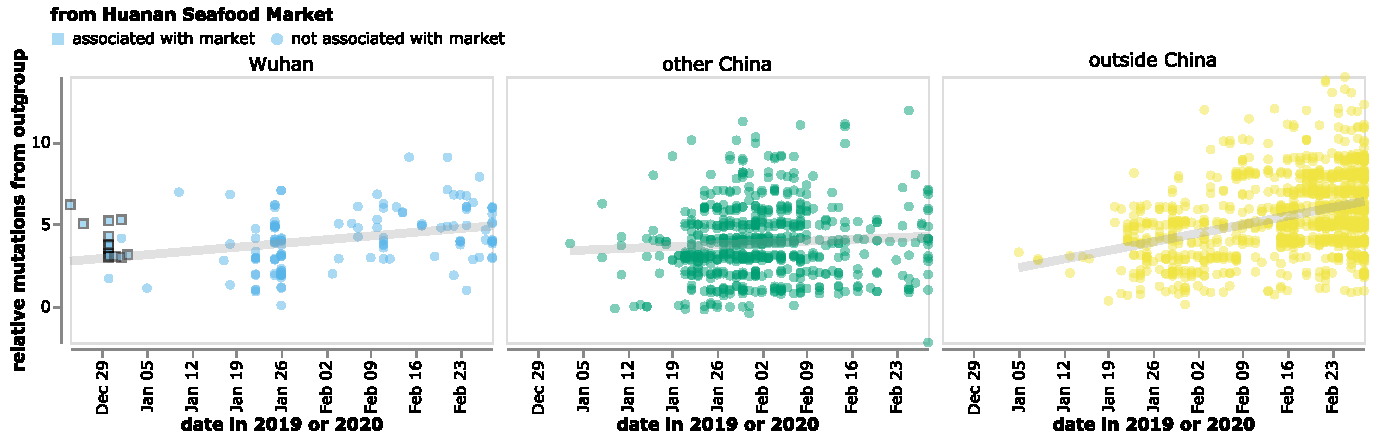
\includegraphics[width=\linewidth]{figures/deltadist_RaTG13.pdf}
\caption{The reported collection dates of SARS-CoV-2 sequences in GISAID versus their relative mutational distances from the RaTG13 bat coronavirus outgroup.
Mutational distances are relative to the putative progenitor proCoV2 inferred by \citet{kumar2021evolutionary}.
The plot shows sequences in GISAID collected no later than February 28, 2020.
Sequences that the joint WHO-China report~\citep{WHO2021origins} describes as being associated with the Wuhan Seafood Market are plotted with squares.
Points are slightly jittered on the y-axis.
Go to {\color{red} add link} for an interactive version of this plot that enables toggling of the outgroup to RpYN06 and RmYN02, mouseovers to see details for each point including strain name and mutations relative to proCoV2, and adjustment of the y-axis jittering.
Static versions of the plot with RpYN06 and RmYN02 outgroups are in Figure~\ref{suppfig:deltadist_RpYN06_RmYN02}.
}
\label{fig:deltadist_RaTG13}
\end{figure*}

This conundrum is illustrated in Figure~\ref{fig:deltadist_RaTG13}, which plots the collection date of SARS-CoV-2 sequences in GISAID versus the relative number of mutational differences from RaTG13~\citep{zhou2020pneumonia}, which is the bat coronavirus with the highest full-genome sequence identity to SARS-CoV-2.
The earliest SARS-CoV-2 sequences were collected in Wuhan in December, but these sequences are more distant from RaTG13 than sequences collected in January from other locations in China or even other countries (Figure~\ref{fig:deltadist_RaTG13}).
The discrepancy is especially pronounced for early Wuhan sequences from patients who had visited the Huanan Seafood Market, which was widely reported as an initial epicenter of the outbreak and has been postulated to be a location of potential zoonosis~\citep{WHO2021origins}.
All sequences associated with the Huanan Seafood Market differ from RaTG13 by at least three more mutations than sequences subsequently collected at various other locations (Figure~\ref{fig:deltadist_RaTG13})---a fact that is difficult to reconcile with the idea that the market was the original location of spread of a bat coronavirus into humans.
Importantly, all these observations also hold true if SARS-CoV-2 is compared to other related bat coronaviruses~\citep{lytras2021exploring} such as RpYN06~\citep{zhou2021identification} or RmYN02~\citep{zhou2020novel} rather than RaTG13 (Figure~\ref{suppfig:deltadist_RpYN06_RmYN02}).

 \begin{figure*}
 \centerline{
 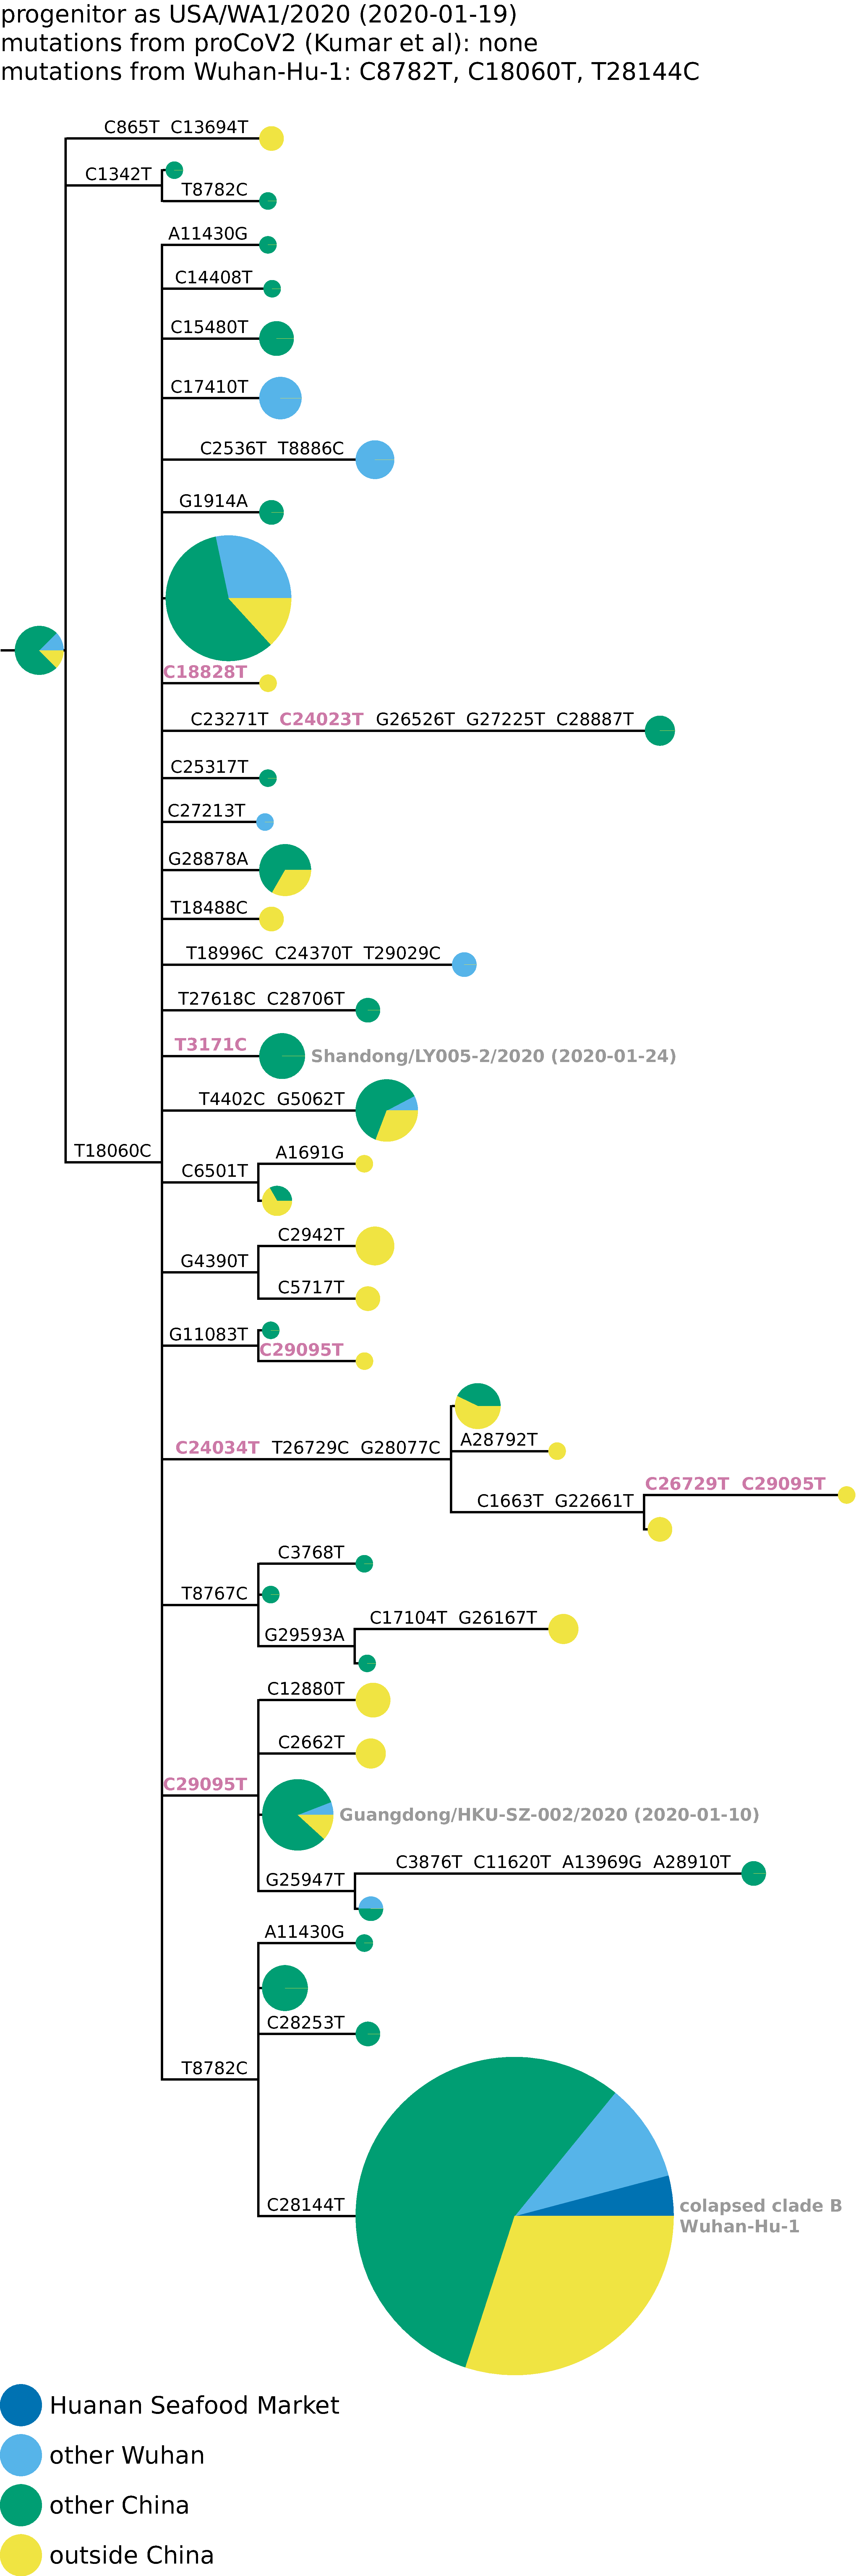
\includegraphics[width=0.31\linewidth, valign=t, clip=true, trim=0in 4.4in 0in 0in]{figures/tree_images/hCoV-19-USA-WA1-2020_RaTG13_without_deleted_seqs.pdf}
 \hspace{0.02\linewidth}
 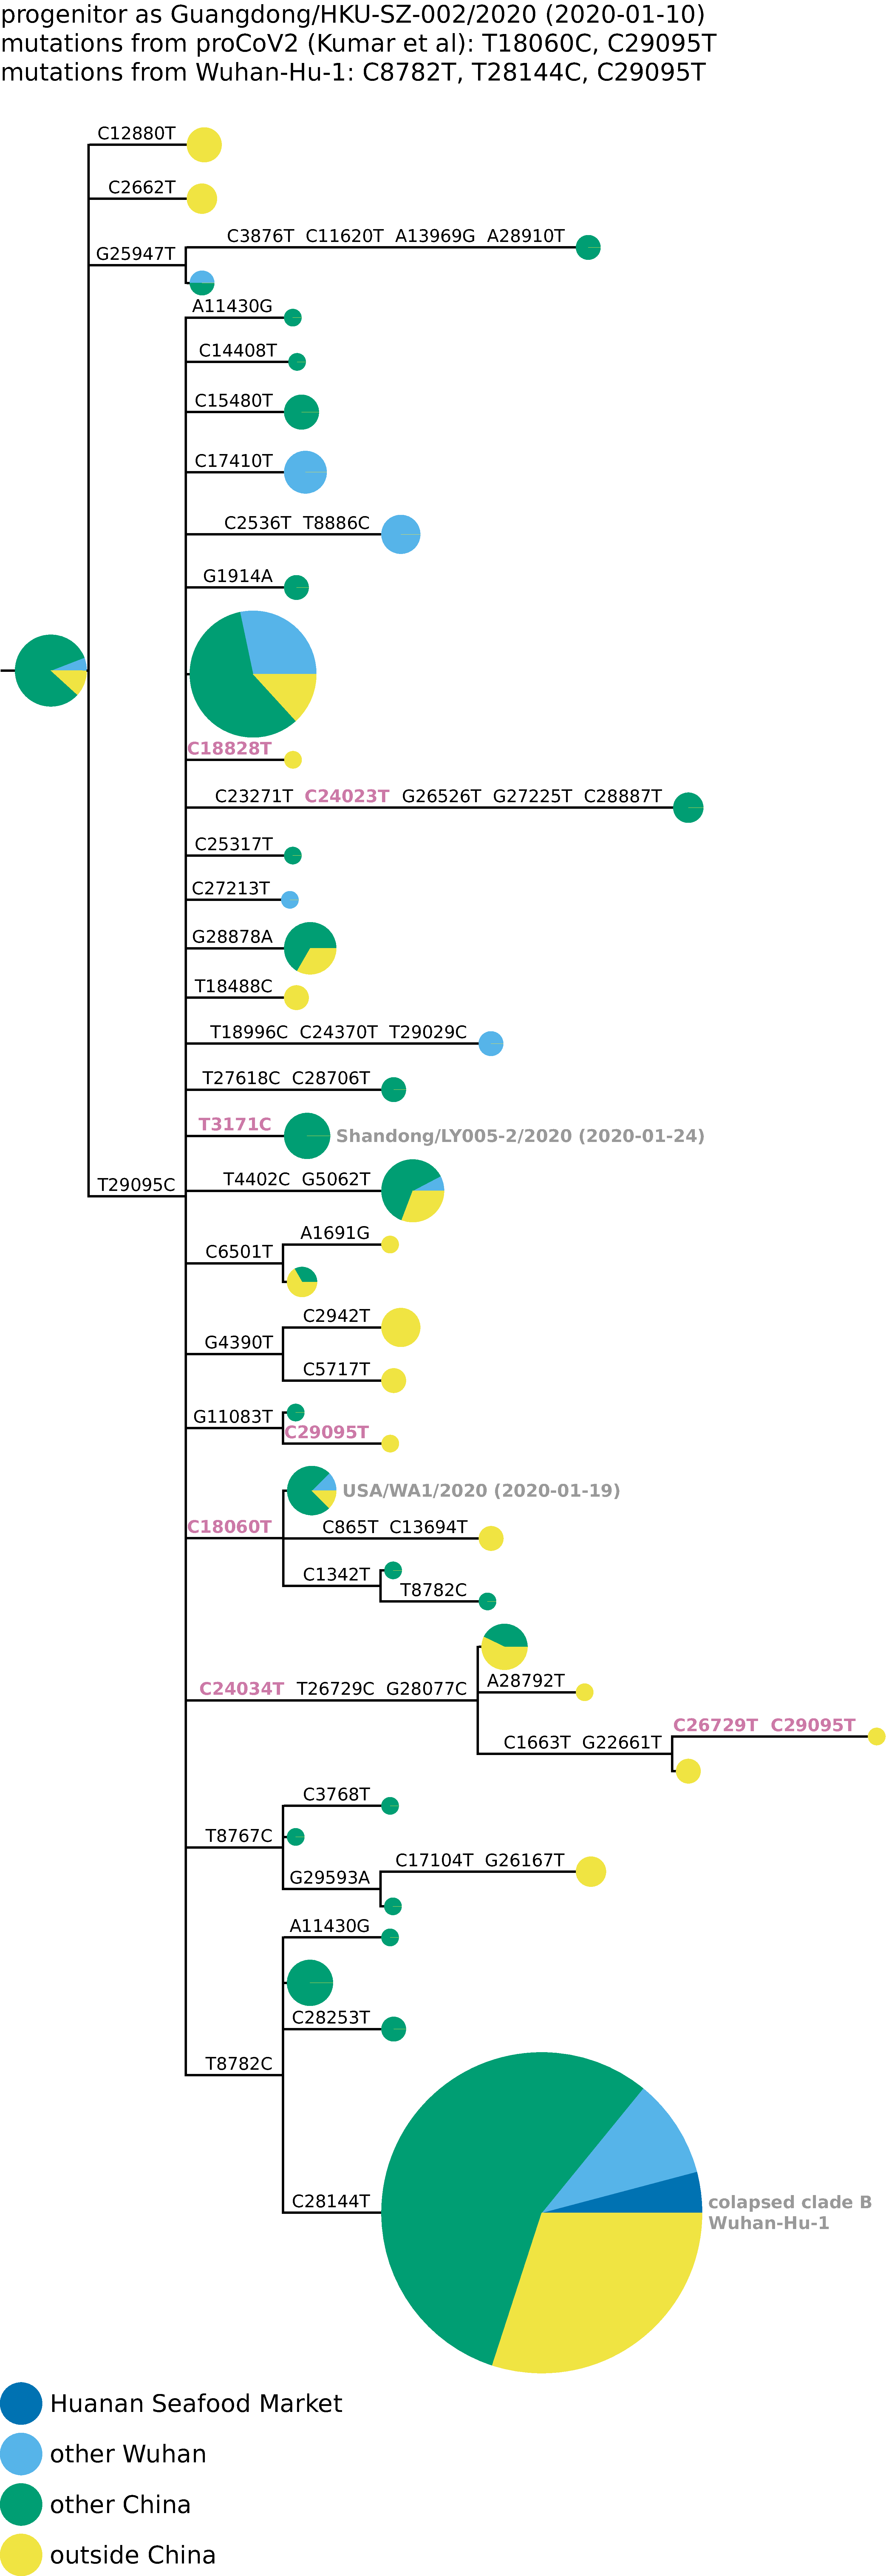
\includegraphics[width=0.33\linewidth, valign=t, clip=true]{figures/tree_images/hCoV-19-Guangdong-HKU-SZ-002-2020_RaTG13_without_deleted_seqs.pdf}
  \hspace{0.02\linewidth}
 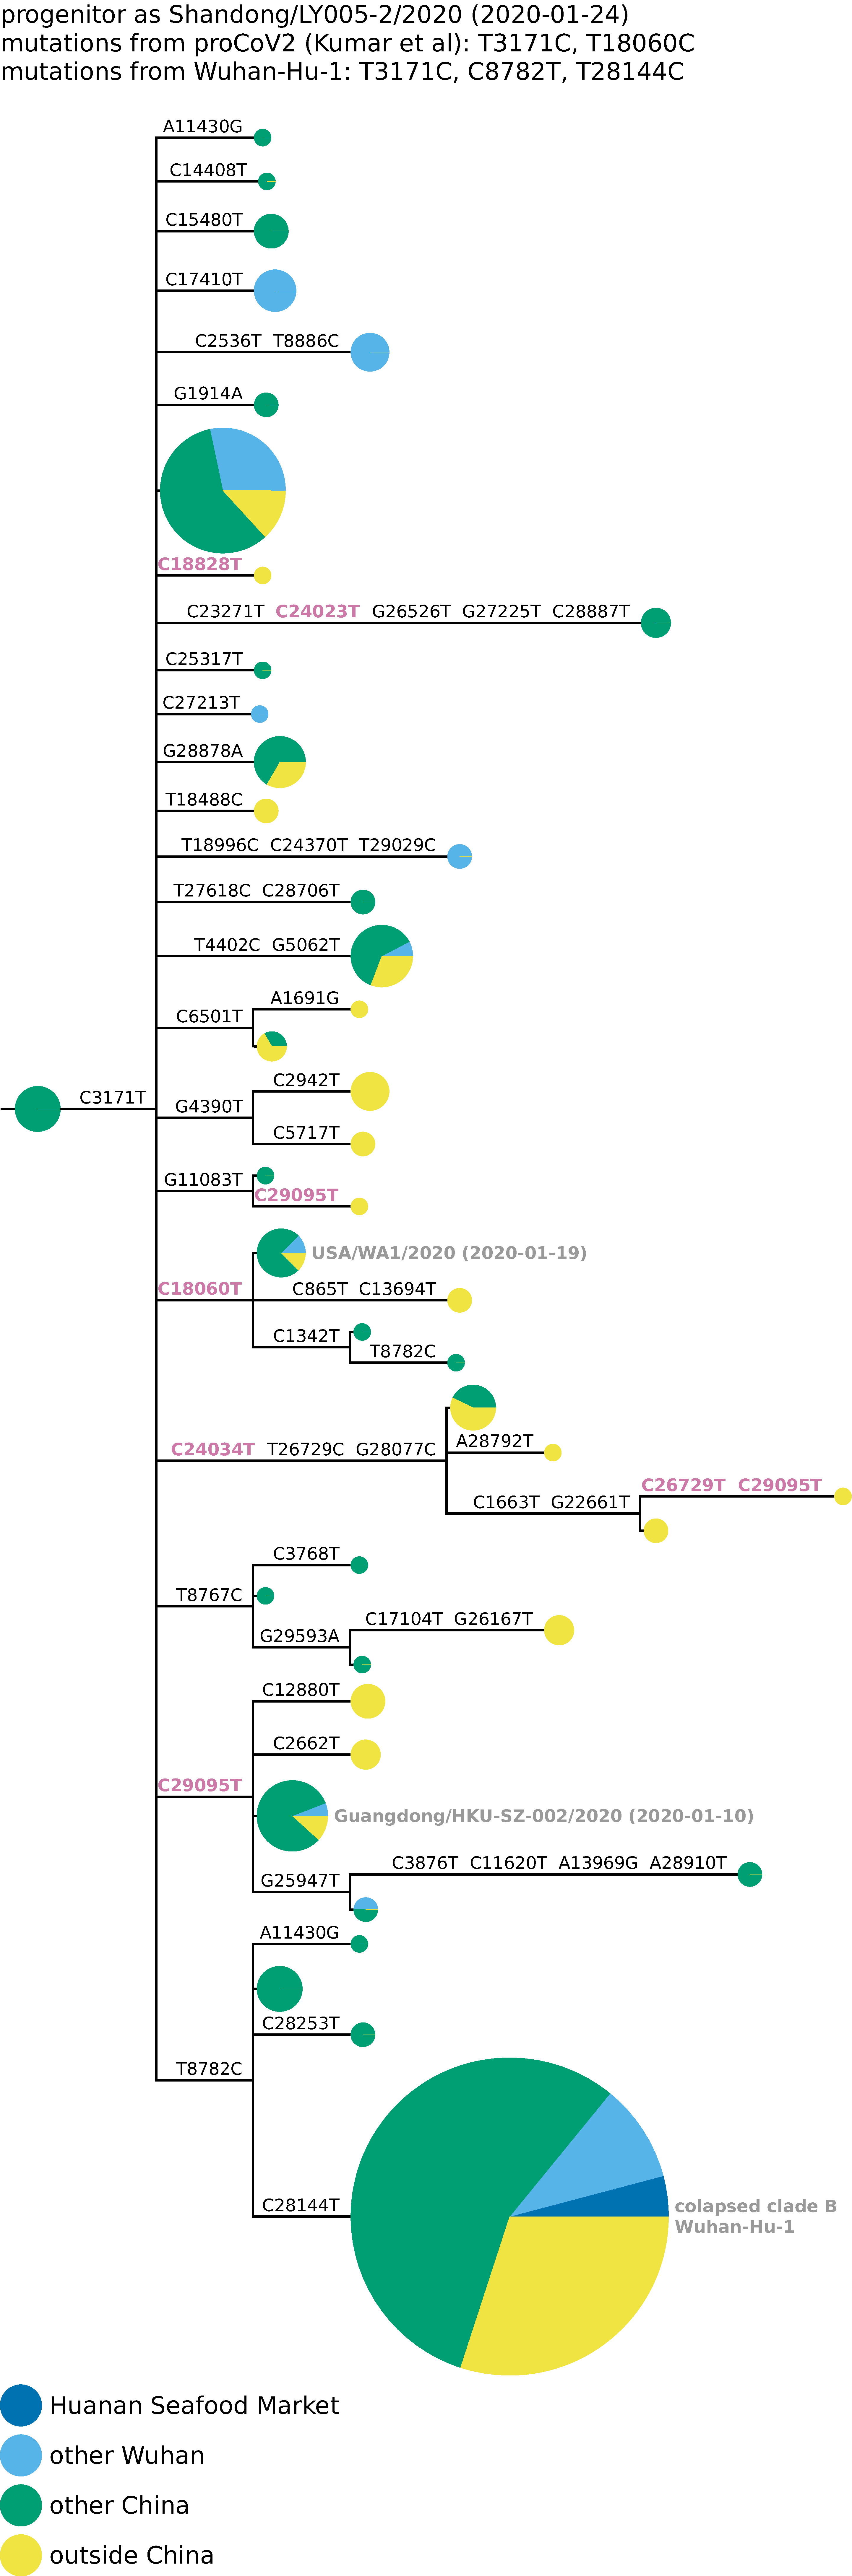
\includegraphics[width=0.31\linewidth, valign=t, clip=true, trim=0in 4.4in 0in 0in]{figures/tree_images/hCoV-19-Shandong-LY005-2-2020_RaTG13_without_deleted_seqs.pdf}
 }
 \caption{
 Phylogenetic trees of all existing SARS-CoV-2 sequences in GISAID with multiple observations among viruses collected no later than January 31, 2020.
 The three trees are identical except they are rooted to make the putative progenitor each of the three sequences with the highest identity to the RaTG13 bat coronavirus outgroup.
Nodes are shown as pie charts with areas proportional to the number of observations of that sequence, and colored by where the viruses were collected (see key at bottom).
The mutations on each branch are labeled, with mutations towards the nucleotide identity in the RaTG13 outgroup in purple.
The labels at the top of each tree show the first known virus identical to each putative progenitor, as well as mutations in that progenitor relative to proCoV2~\citep{kumar2021evolutionary} and the Wuhan-Hu-1 reference sequence.
All sequences in the monophyletic group containing C28144T are collapsed into a single node labeled ``clade B'' in concordance with the naming scheme of \citet{rambaut2020dynamic}; this clade contains Wuhan-Hu-1.
 Figure~\ref{suppfig:tree_RpYN06_RmYN02} shows that identical results are obtained if the outgroup is instead RpYN06 or RmYN02.
\label{fig:tree_RaTG13}
 }
 \end{figure*}

This conundrum can also be visualized in a phylogenetic context by rooting a tree of early SARS-CoV-2 sequences so that the ``progenitor'' sequence is closest to the bat coronavirus outgroup.
If we limit the analysis to sequences with at least two observations among strains collected no later than January 2020, there are three ways to root the tree in this fashion since there are three different sequences equally close to the bat coronavirus outgroup (Figure~\ref{fig:tree_RaTG13}, Figure~\ref{suppfig:tree_RpYN06_RmYN02}).
Importantly, none of these rootings place any Huanan Seafood Market viruses (or other Wuhan viruses from December 2019) in the progenitor node---and only one of the three rootings has any virus from Wuhan in the progenitor node (in the leftmost tree in Figure~\ref{fig:tree_RaTG13}, the progenitor node contains Wuhan/0126-C13/2020, which is reported to have been collected on January 26, 2020).
Therefore, inferences about the progenitor of SARS-CoV-2 based on comparison to related bat viruses are inconsistent with inferences based on the dates of sequence collection and epidemiological evidence suggesting Wuhan was the origin of the pandemic~\citep{pipes2021assessing}.

Several plausible explanations have been proposed for the discordance of phylogenetic rooting with evidence that Wuhan was the origin of the pandemic.
\citet{rambaut2020dynamic} suggest that viruses from the clade labeled ``B'' in Figure~\ref{fig:tree_RaTG13} may just ``happen'' to have been sequenced first, but that other SARS-CoV-2 sequences are really more ancestral as implied by phylogenetic rooting.
\citet{pipes2021assessing} provide a detailed discussion of the conundrum, and suggest that phylogenetic rooting could be incorrect due to technical reasons such as high divergence of the outgroup or unusual mutational processes not captured in substitution models.
\citet{kumar2021evolutionary} agree that phylogenetic rooting is problematic, and circumvent this problem by using an alternative algorithm to infer a progenitor for SARS-CoV-2 that they name proCoV2.
Notably, proCoV2 turns out to be identical to one of the putative progenitors yielded by my approach in Figure~\ref{fig:tree_RaTG13} of simply placing the root at the nodes closest to the bat outgroup.
However, neither the sophisticated algorithm of \citet{kumar2021evolutionary} nor my more simplistic approach in Figure~\ref{fig:tree_RaTG13} explain \emph{why} the progenitor should be so different from the earliest sequences reported from Wuhan.

Before moving onto the next section, I will also briefly address two less plausible explanations for the discordance between phylogenetic rooting and epidemiological data that have gained traction in discussion of SARS-CoV-2's origins.
The first explanation, which has circulated on social media, suggests that the RaTG13 sequence might be faked in a way that confounds phylogenetic inference of SARS-CoV-2's progenitor.
This explanation can be discounted, because although there are unusual aspects of RaTG13's primary sequencing data~\citep{singla2020novo,rahalkar2020anomalous}, the conundrum about inferring the progenitor holds for other outgroups such as RpYN06, RmYN02, and more distant bat coronaviruses reported before emergence of SARS-CoV-2 such as ZC45~\citep{tang2020origin}.
The second explanation, which was proposed in a blog post by \citet{garry2021early} and amplified by a popular podcast~\citep{twiv2021}, is that there were multiple zoonoses from distinct markets, with the Huanan Seafood Market being the source of viruses in clade B, and some other unknown market being the source of viruses that lack the T8782C and C28144T mutations.
However, inspection of the phylogenetic trees in Figure~\ref{fig:tree_RaTG13} shows this idea can also be discounted: clade B is connected to viruses lacking T8782C and C28144T by single mutational steps via other human isolates, so this explanation requires not only positing two markets with two progenitors differing by just two mutations, but then also the exceedingly improbable evolution of one of these progenitors towards the other after it had jumped to humans.

\subsection{Sequences recovered from the deleted project help resolve inferences about SARS-CoV-2's progenitor}
To examine if the sequences recovered from the deleted data set help resolve the conundrum described in the previous section, I repeated the analyses including those sequences.
In the process, I noted another salient fact: four GISAID sequences collected in Guangdong that fall in a putative progenitor node are from patients who traveled to Wuhan in late December of 2019 and developed symptoms before or on the day that they returned to Guangdong, where their viruses were ultimately sequenced~\citep{chan2020familial, kang2020evidence}.
Since these patients were clearly infected in Wuhan even though they were sequenced in Guangdong, I annotated them separately from both the other Wuhan and other China sequences.

\begin{figure}
\centering
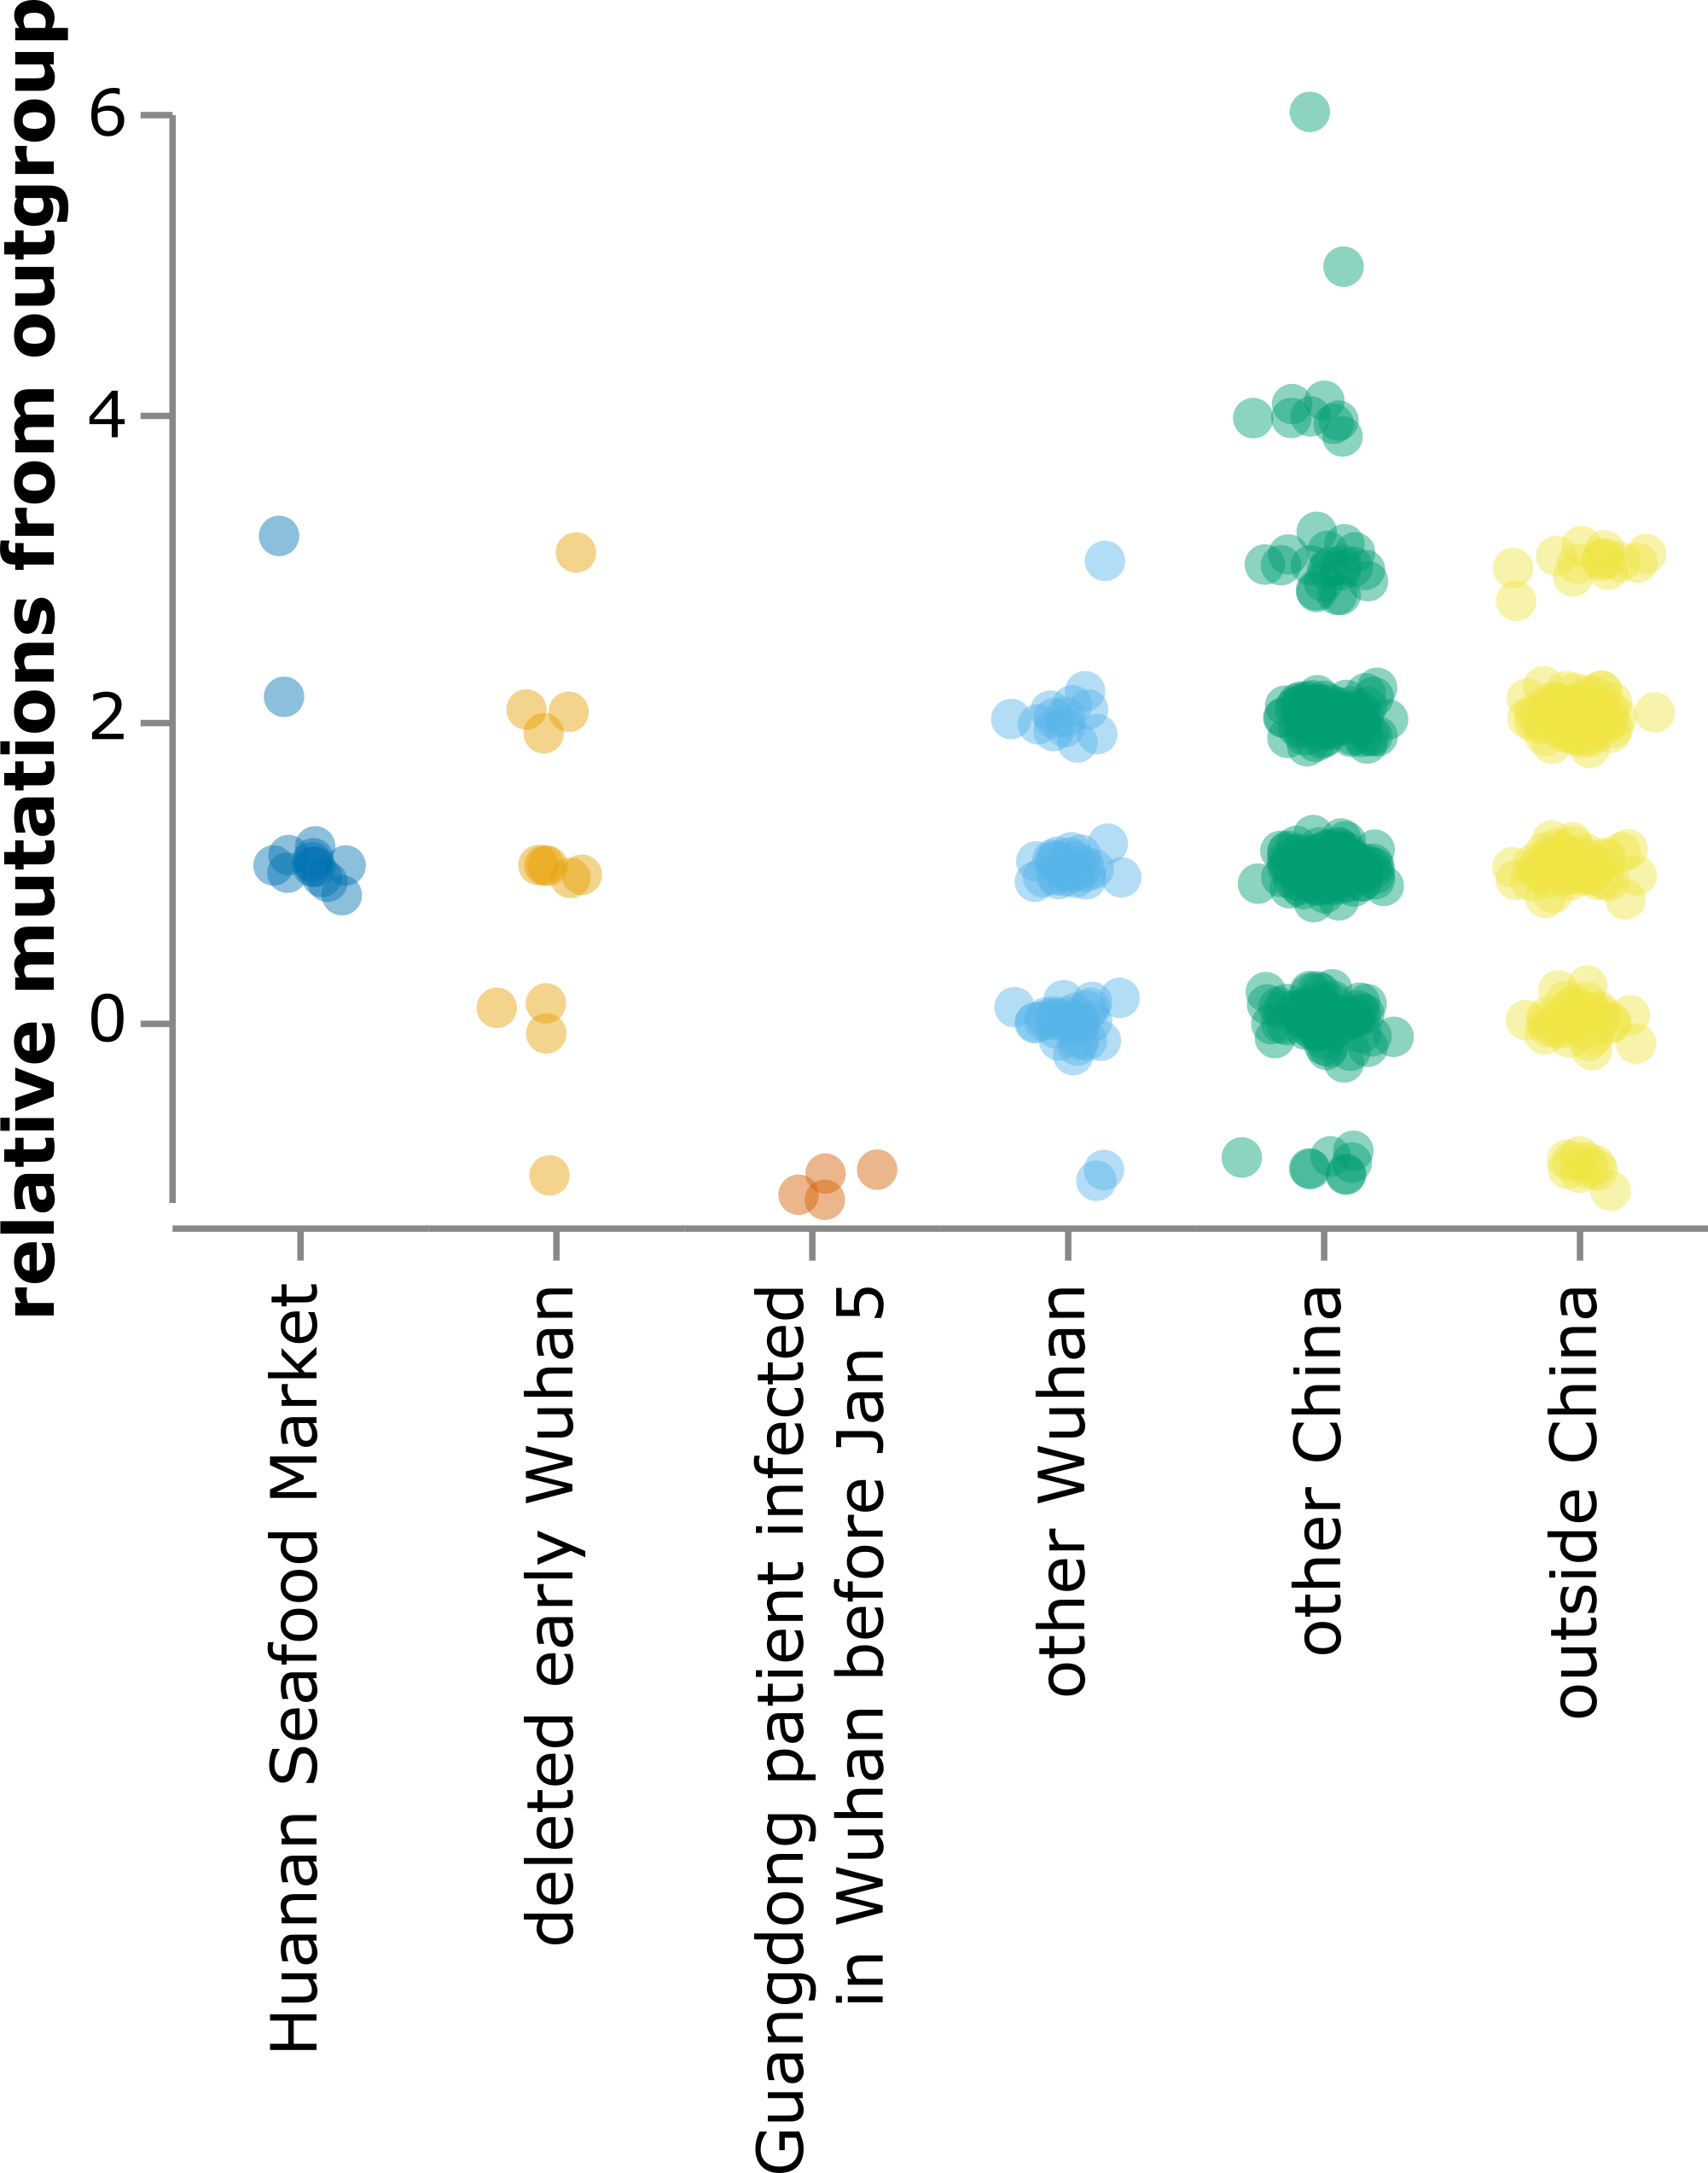
\includegraphics[width=0.75\linewidth]{figures/deltadist_jitter.png}
\caption{
Relative mutational distance from RaTG13 bat coronavirus outgroup calculated \emph{only} over the region of the SARS-CoV-2 genome covered by the sequences recovered from the deleted data set (sites 21,570--29,550).
The plot shows sequences in GISAID collected before February of 2020, as well as the 13 early Wuhan epidemic sequences in Table~\ref{tab:mutations}.
Mutational distance is calculated relative to proCoV2, and points are slightly jittered on the y-axis.
Go to {\color{red} add link} for an interactive version of this plot that enables toggling the outgroup to RpYN06 or RmYN02, mouseovers to see details for each point, and adjustment of y-axis jittering.
\label{fig:deltadist_jitter}
}
\end{figure}

 \begin{figure*}
 \centerline{
 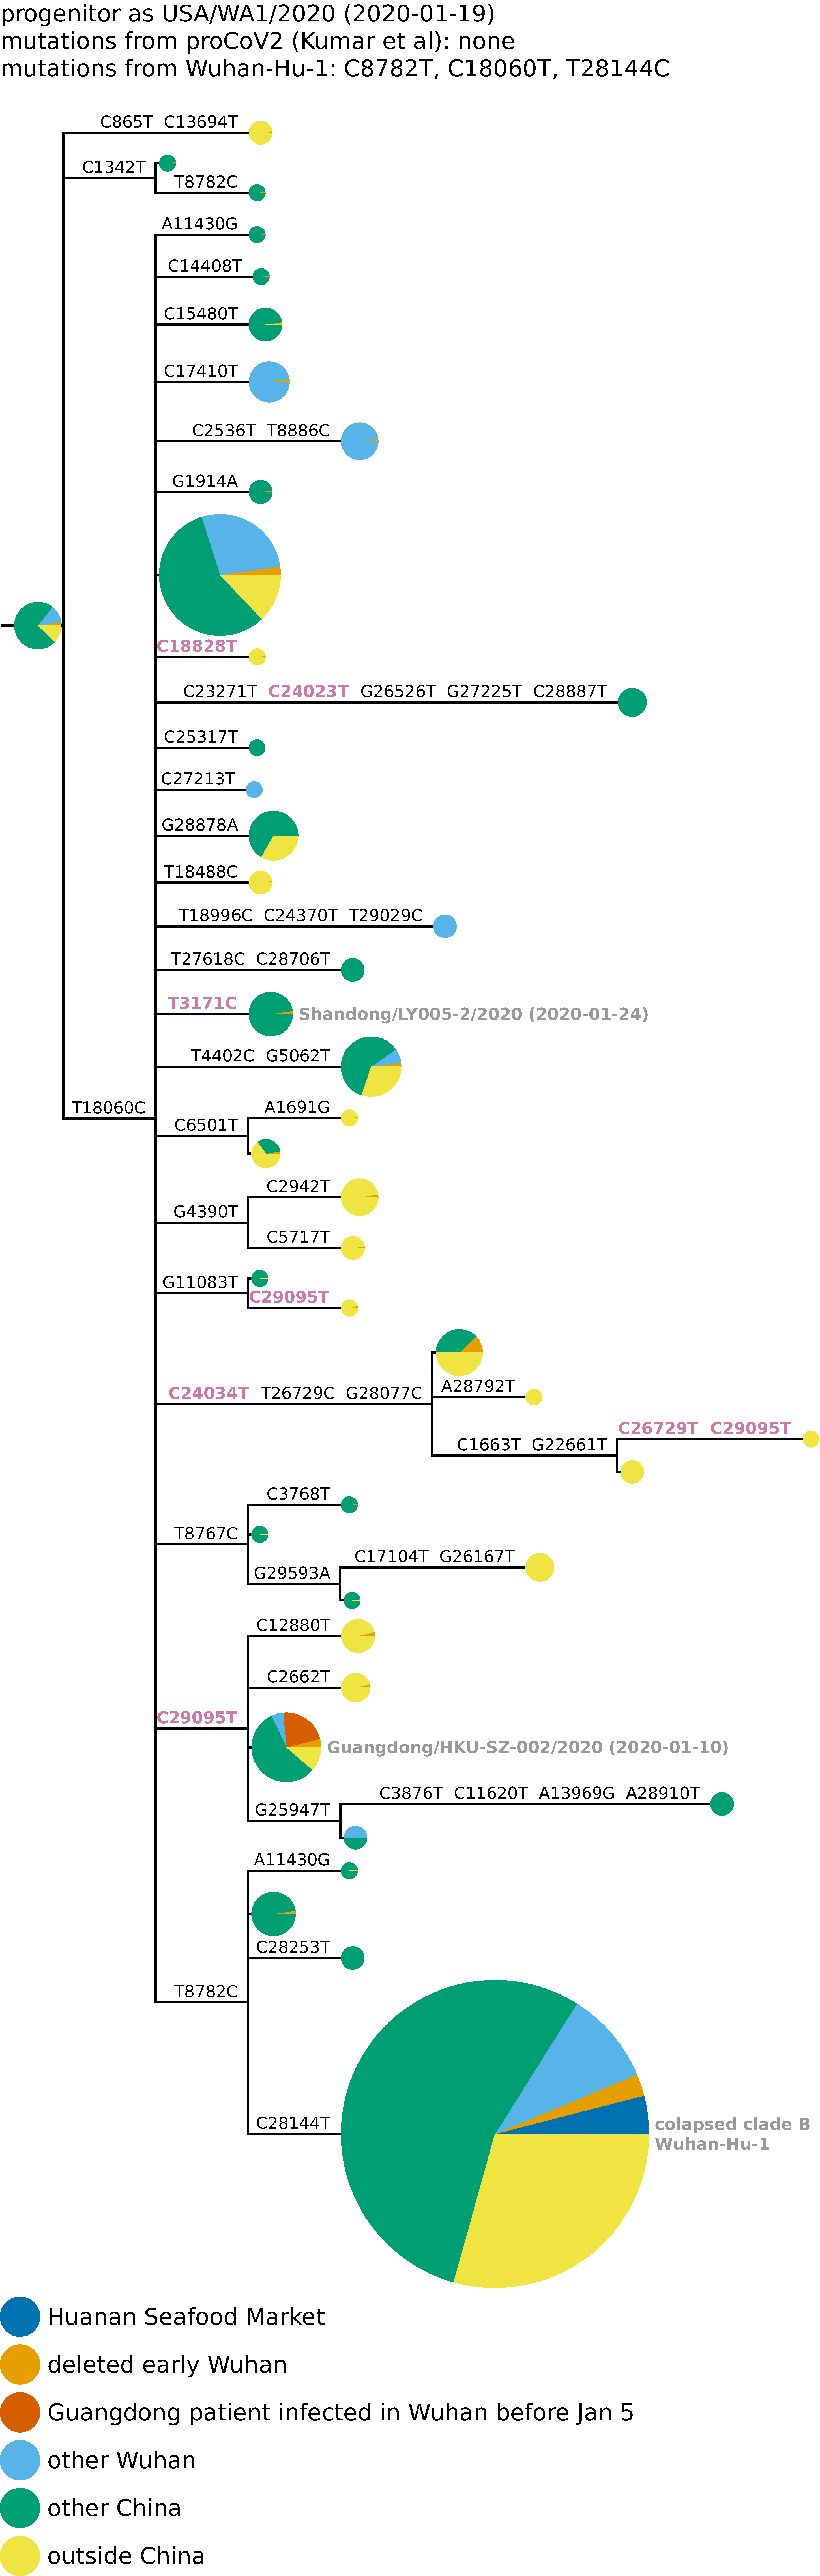
\includegraphics[width=0.31\linewidth, valign=t, clip=true, trim=0in 6.75in 0in 0in]{figures/tree_images/hCoV-19-USA-WA1-2020_RaTG13_with_deleted_seqs.pdf}
 \hspace{0.02\linewidth}
 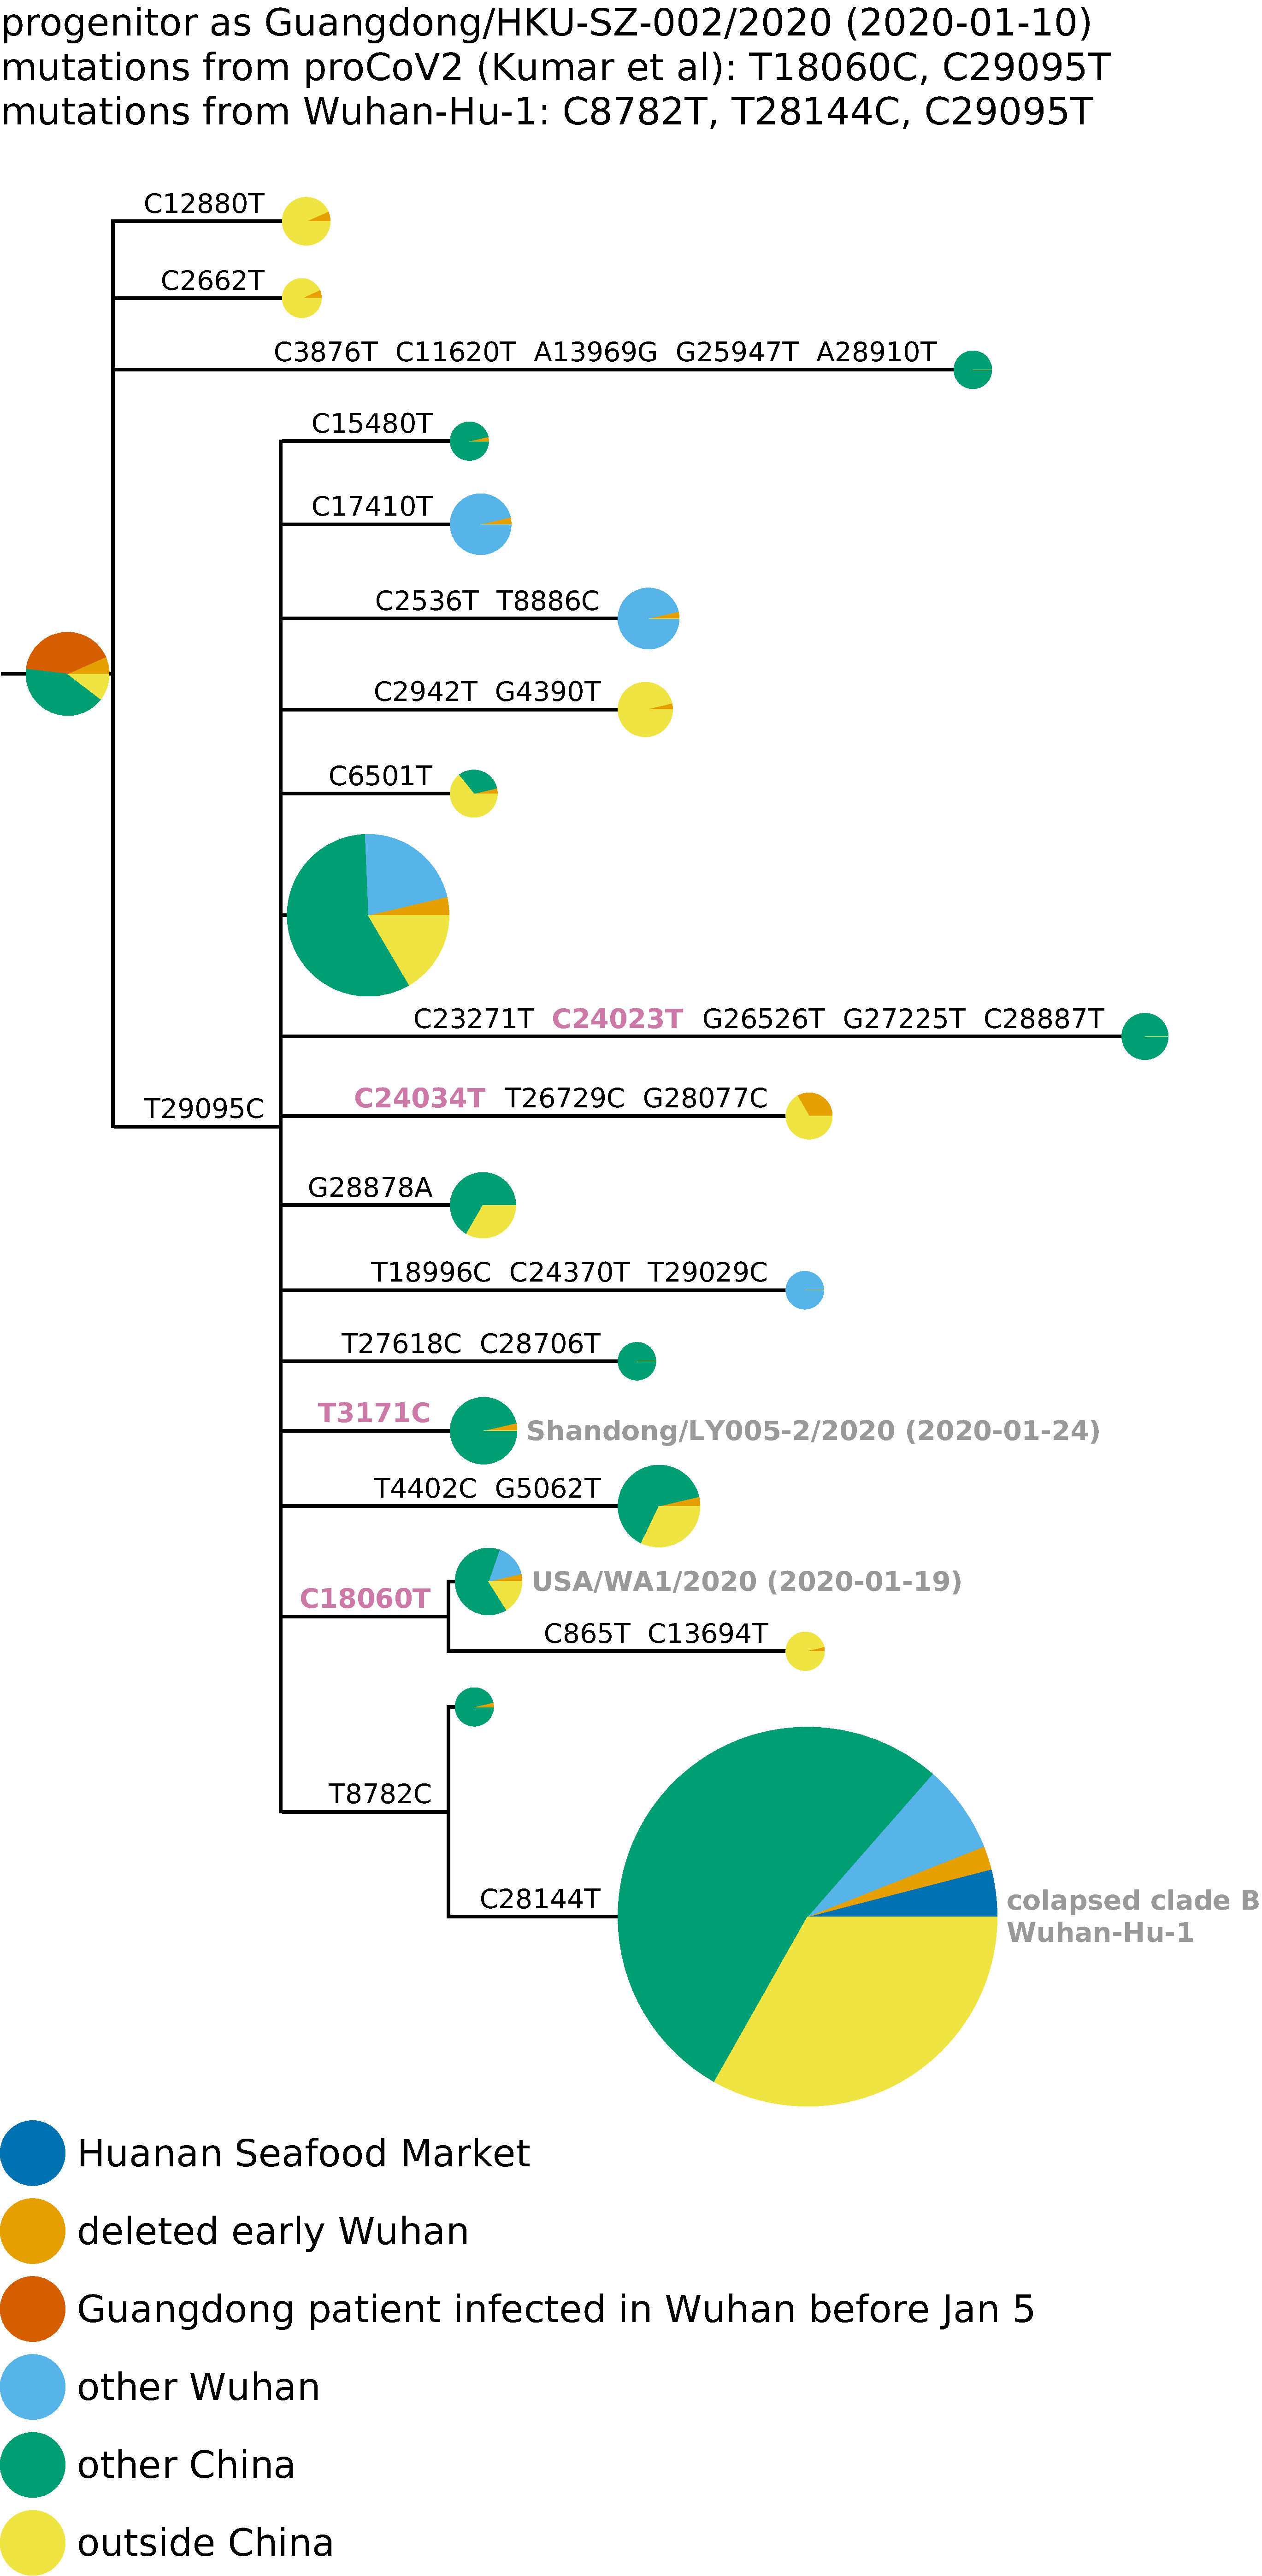
\includegraphics[width=0.33\linewidth, valign=t, clip=true]{figures/tree_images/hCoV-19-Guangdong-HKU-SZ-002-2020_RaTG13_with_deleted_seqs.pdf}
  \hspace{0.02\linewidth}
 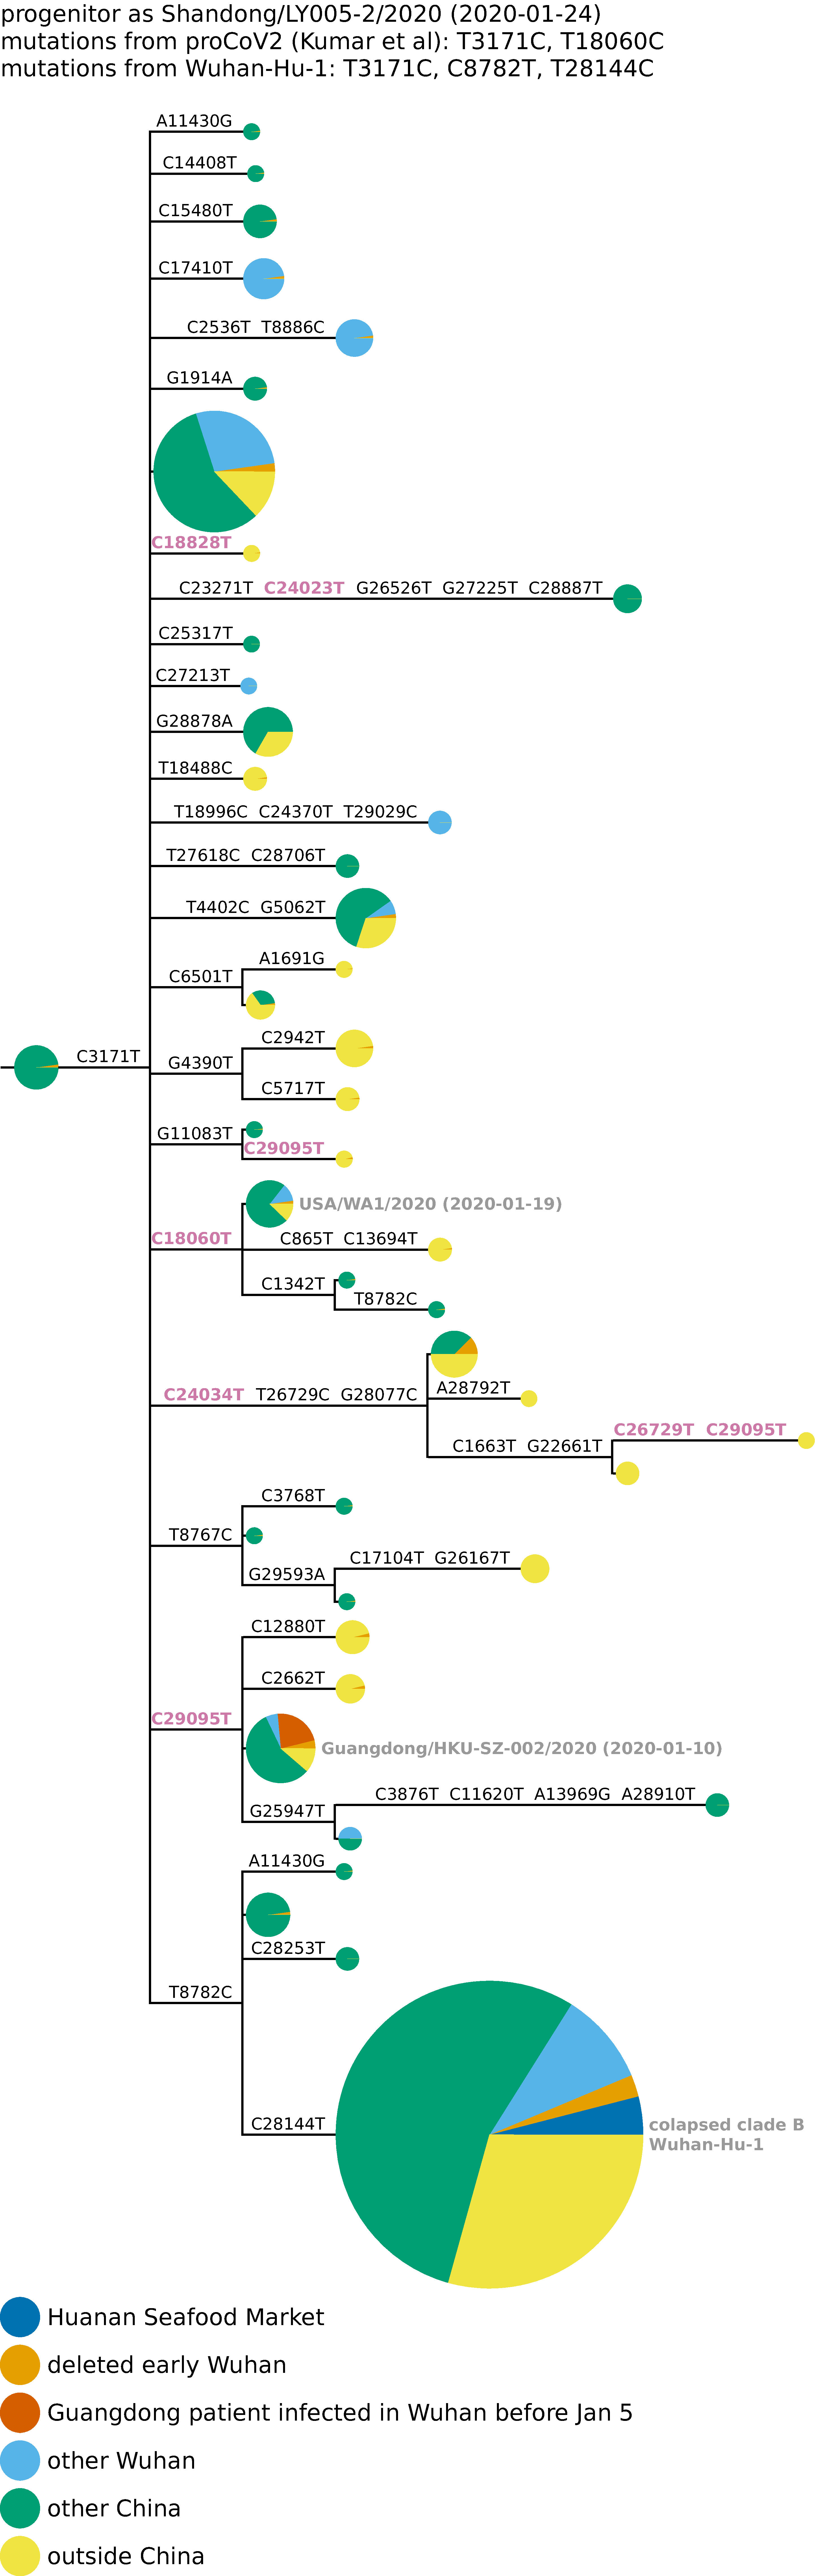
\includegraphics[width=0.31\linewidth, valign=t, clip=true, trim=0in 6.75in 0in 0in]{figures/tree_images/hCoV-19-Shandong-LY005-2-2020_RaTG13_with_deleted_seqs.pdf}
 }
 \caption{
Phylogenetic trees identical to those in Figure~\ref{fig:tree_RaTG13} except with the addition of the early Wuhan epidemic sequences from the deleted data set, and with Guangdong patients infected in Wuhan prior to January 5 annotated separately.
Because the deleted data set only provides partial sequences, they cannot all be placed unambiguously on the tree.
Therefore, they are added to each node with which they are compatible proportional to the number of sequences already in that node.
The sequences with C28144T (clade B) or C29095T (putative progenitor in middle tree) can be placed relatively unambiguously as key lineage-defining mutations occur in the sequenced region, but the sequences that lack either of these mutations can be placed in a large number of nodes including that of the proCoV2 putative progenitor.
 Figure~\ref{suppfig:tree_RpYN06_RmYN02} has already demonstrated that the results are identical if RpYN06 or RmYN02 are instead used as the outgroup.
\label{fig:tree_with_deleted}
 }
 \end{figure*}

Several of the early epidemic sequences from the deleted project and all of the sequences from patients infected in Wuhan but sequenced in Guangdong were more similar to the bat coronavirus outgroup than any sequences from the Huanan Seafood Market across the region in which all were fully sequenced (Figure~\ref{fig:deltadist_jitter}).
To place this observation in a phylogenetic context, I added the deleted sequences at compatible locations to the full-genome phylogenetic trees described in the previous section (Figure~\ref{fig:tree_with_deleted}).

It is immediately apparent that the discrepancy between outgroup rooting and epidemiological evidence that Wuhan was the origin of SARS-CoV-2 is alleviated by adding the deleted sequences and annotating Wuhan infections sequenced in Guangdong (Figure~\ref{fig:tree_with_deleted}).
The middle tree in Figure~\ref{fig:tree_with_deleted} now looks highly plausible, as half its progenitor node is derived from early Wuhan infections, which is more than any other equivalently large node.
The first known sequence identical to this putative progenitor (Guangdong/HKU-SZ-002/2020) is from a patient who developed symptoms on January 4 while visiting Wuhan~\citep{chan2020familial}.
In this scenario, the progenitor has three mutations towards the bat coronavirus outgroup relative to Wuhan-Hu-1 (C8782T, T28144C, and C29095T), and two mutations relative to proCoV2 (T18060C away from the outgroup and C29095T towards the outgroup).
The leftmost tree in Figure~\ref{fig:tree_with_deleted}, which has a putative progenitor identical to proCoV2~\citep{kumar2021evolutionary} also looks plausible, with some weight from Wuhan sequences.
Note that although three deleted early epidemic sequences are compatible with this proCoV2 progenitor, the defining C18060T mutation is not covered in the sequenced region---so further sequencing of these samples would be informative.
The rightmost tree in Figure~\ref{fig:tree_with_deleted} looks less plausible, as it has almost no weight from Wuhan and the first sequence identical to its progenitor was not collected until January 24.

We can also qualitatively evaluate the three progenitor placements in Figure~\ref{fig:tree_with_deleted} using the sample principle employed by \citet{worobey2020emergence} to help evaluate scenarios for the emergence of SARS-CoV-2 in Europe and North America: namely that during an exponentially growing outbreak, a progenitor is likely to give rise to multiple distinct branching lineages.
This principle is especially likely to hold for the scenarios represented in Figure~\ref{fig:tree_with_deleted}, where the are multiple observed representatives of each putative progenitor which each have the potential to yield descendants with new mutations.
Using this qualitative idea, the middle scenario in Figure~\ref{fig:tree_with_deleted} seems most plausible, the leftmost (proCoV2) scenario also seems plausible, and the rightmost scenario seems less plausible.
I acknowledge that these arguments are purely qualitative and lack the formal statistical analysis of \citet{worobey2020emergence}---but as discussed below, there may be wisdom in more qualitative reasoning when there are valid concerns about the nature of the underlying data.

\section{Discussion}

Something about lacking formal analyses of some other studies, but maybe this is not so bad.

\section{Methods}

\subsection{Code and data availability}
The deleted SRA files recovered from the Google cloud are all available at  \url{https://github.com/jbloom/SARS-CoV-2_PRJNA612766/tree/main/results/sra_downloads}.
I have suffixed the file extension \texttt{.sra} to all of these files.

\subsection{Archiving of key weblinks}
I have digitally archived key weblinks in the Wayback Machine.
These include:
\begin{itemize}
\item The first supplementary table of \citet{farkas2020insights}, which lists all SARS-CoV-2 accessions in the SRA as of March 30, 2020, is archived at \url{https://web.archive.org/web/20210502130356/https://dfzljdn9uc3pi.cloudfront.net/2020/9255/1/Supplementary_Table_1.xlsx}. 
\end{itemize}

\bibliography{references}

\clearpage
\onecolumn
\renewcommand{\thepage}{S\arabic{page}}
\setcounter{page}{1}
\renewcommand{\thefigure}{S\arabic{figure}}
\setcounter{figure}{1}

\section{Supplementary Material}

\begin{figure}[h!]
\centering
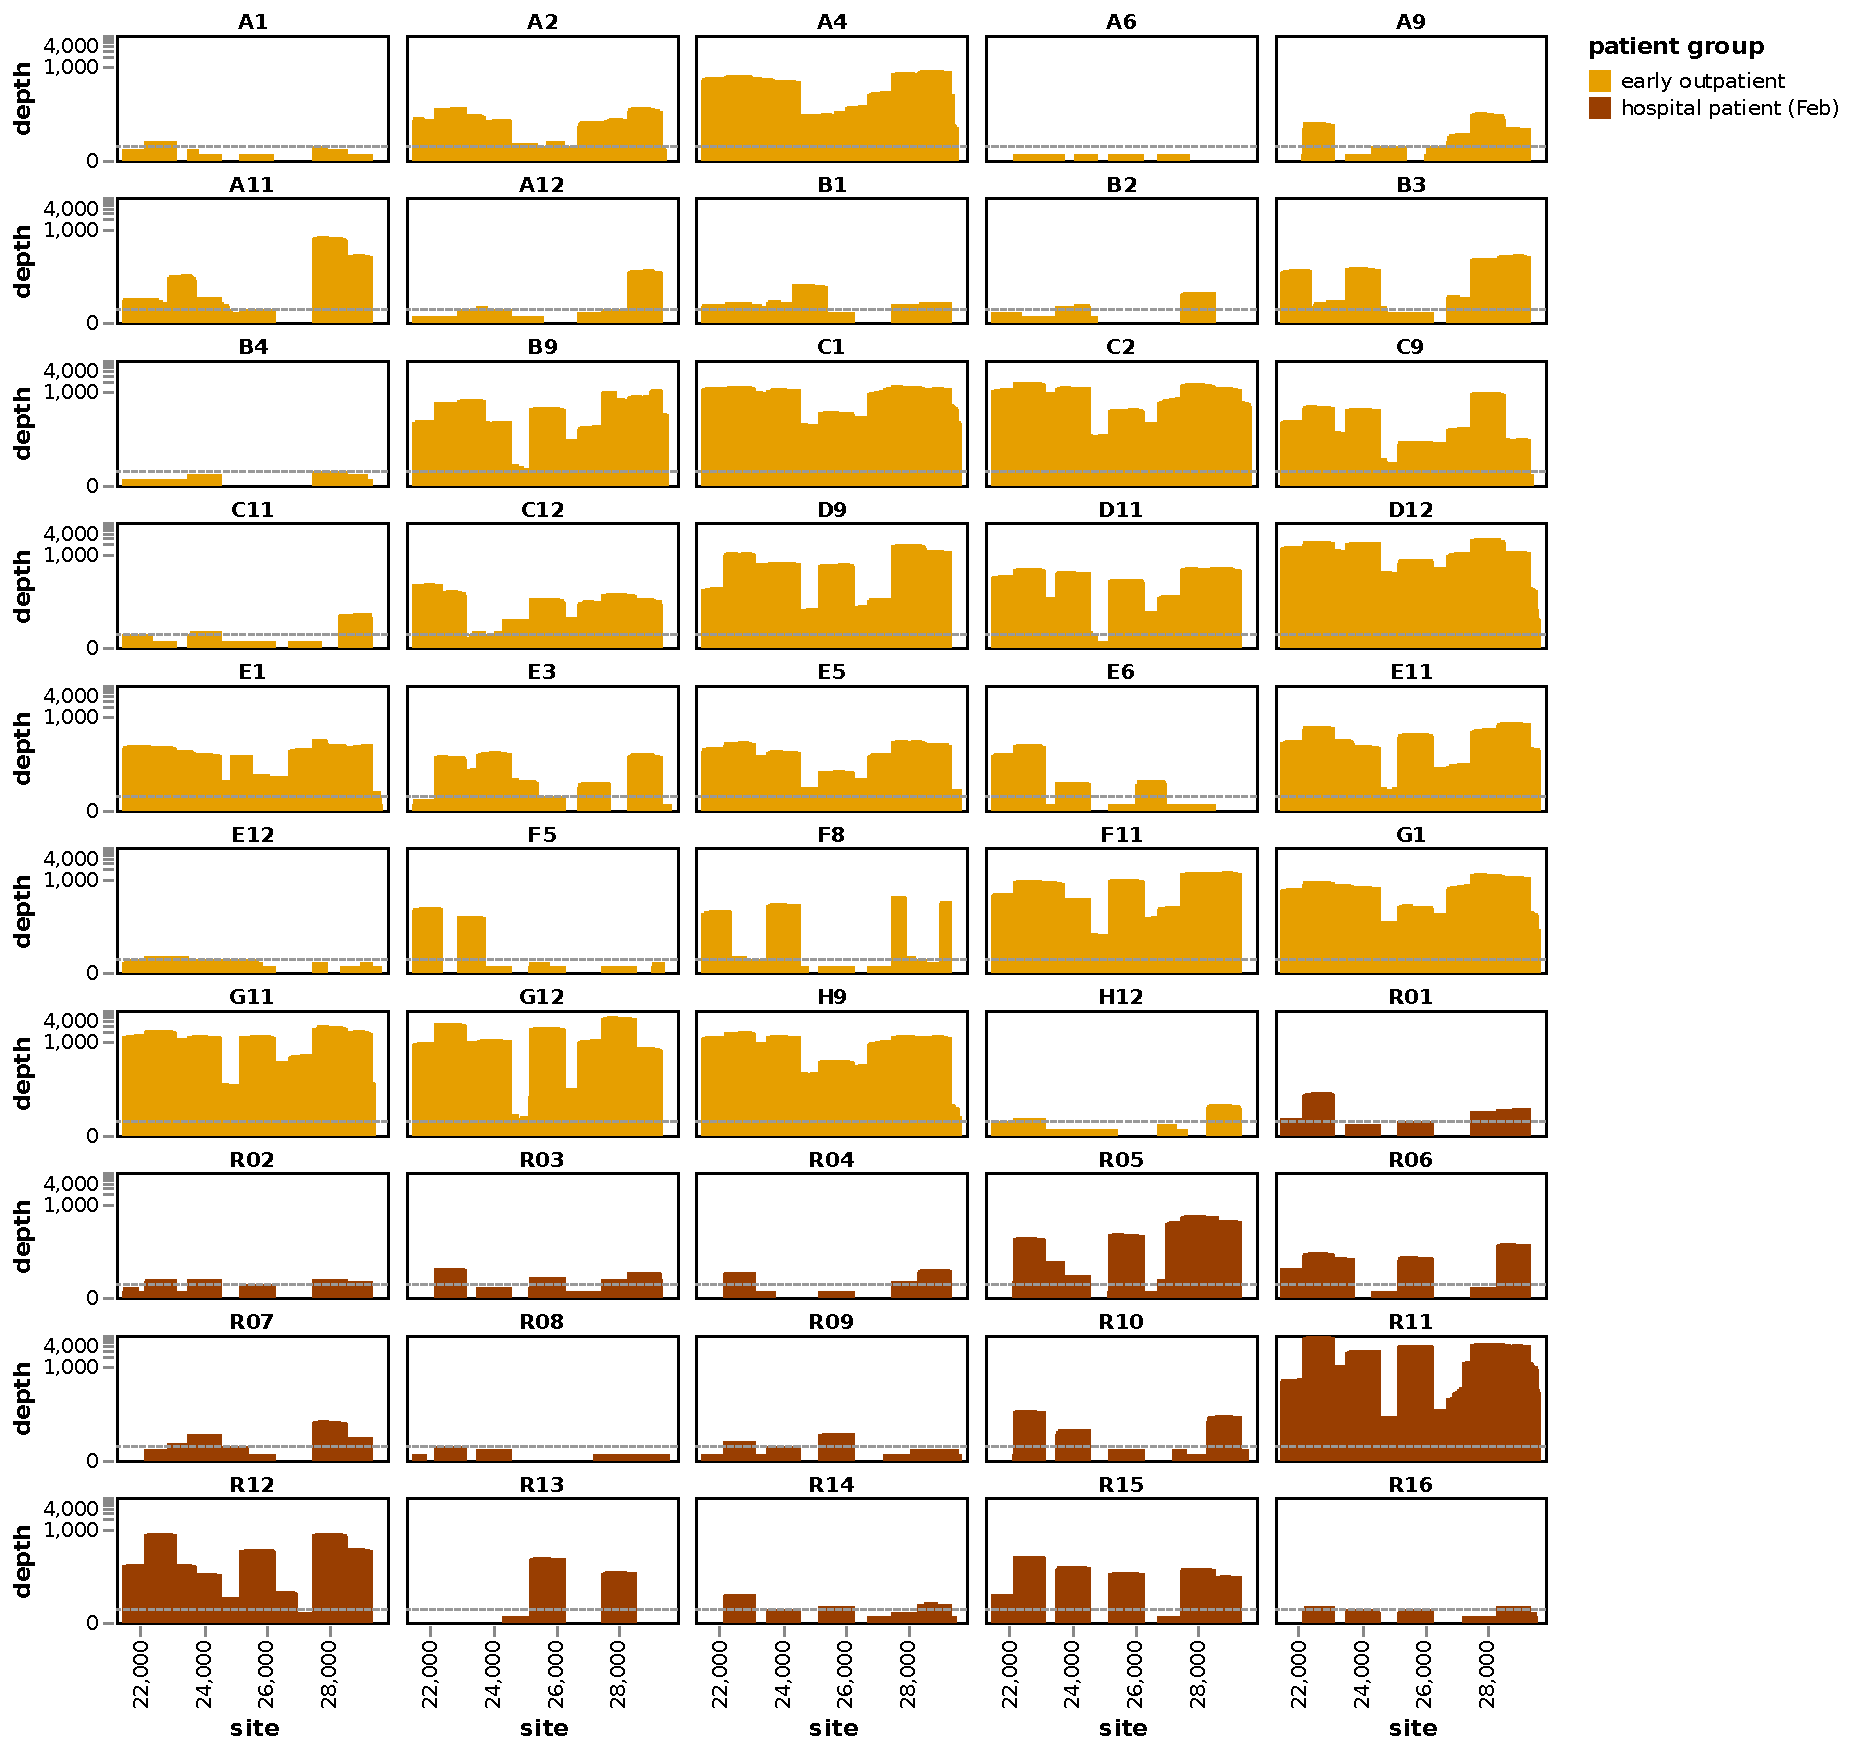
\includegraphics[width=\linewidth]{figures/coverage_region.pdf}
\caption{Sequencing depth over the SARS-CoV-2 genome from site 21,570 to 29,550 for the 34 virus-positive early epidemic samples and the 16 samples from hospitalized patients in February.
Depth is the number of aligned reads that cover that site with a quality score $\ge$20.
The dashed gray line is the minimum coverage required to call a consensus identity at a site.
Note that the y-axis uses a symlog scale.
An interactive version of this plot that enables zooming into specific site ranges and mouseovers to see read count statistics at each site is at {\color{red} add link}.
A version of the plot where the x-axis spans the entire SARS-CoV-2 genome is in Figure~\ref{suppfig:coverage_all}.
}
\label{suppfig:coverage}
\end{figure}

\begin{figure}[h!]
\centering
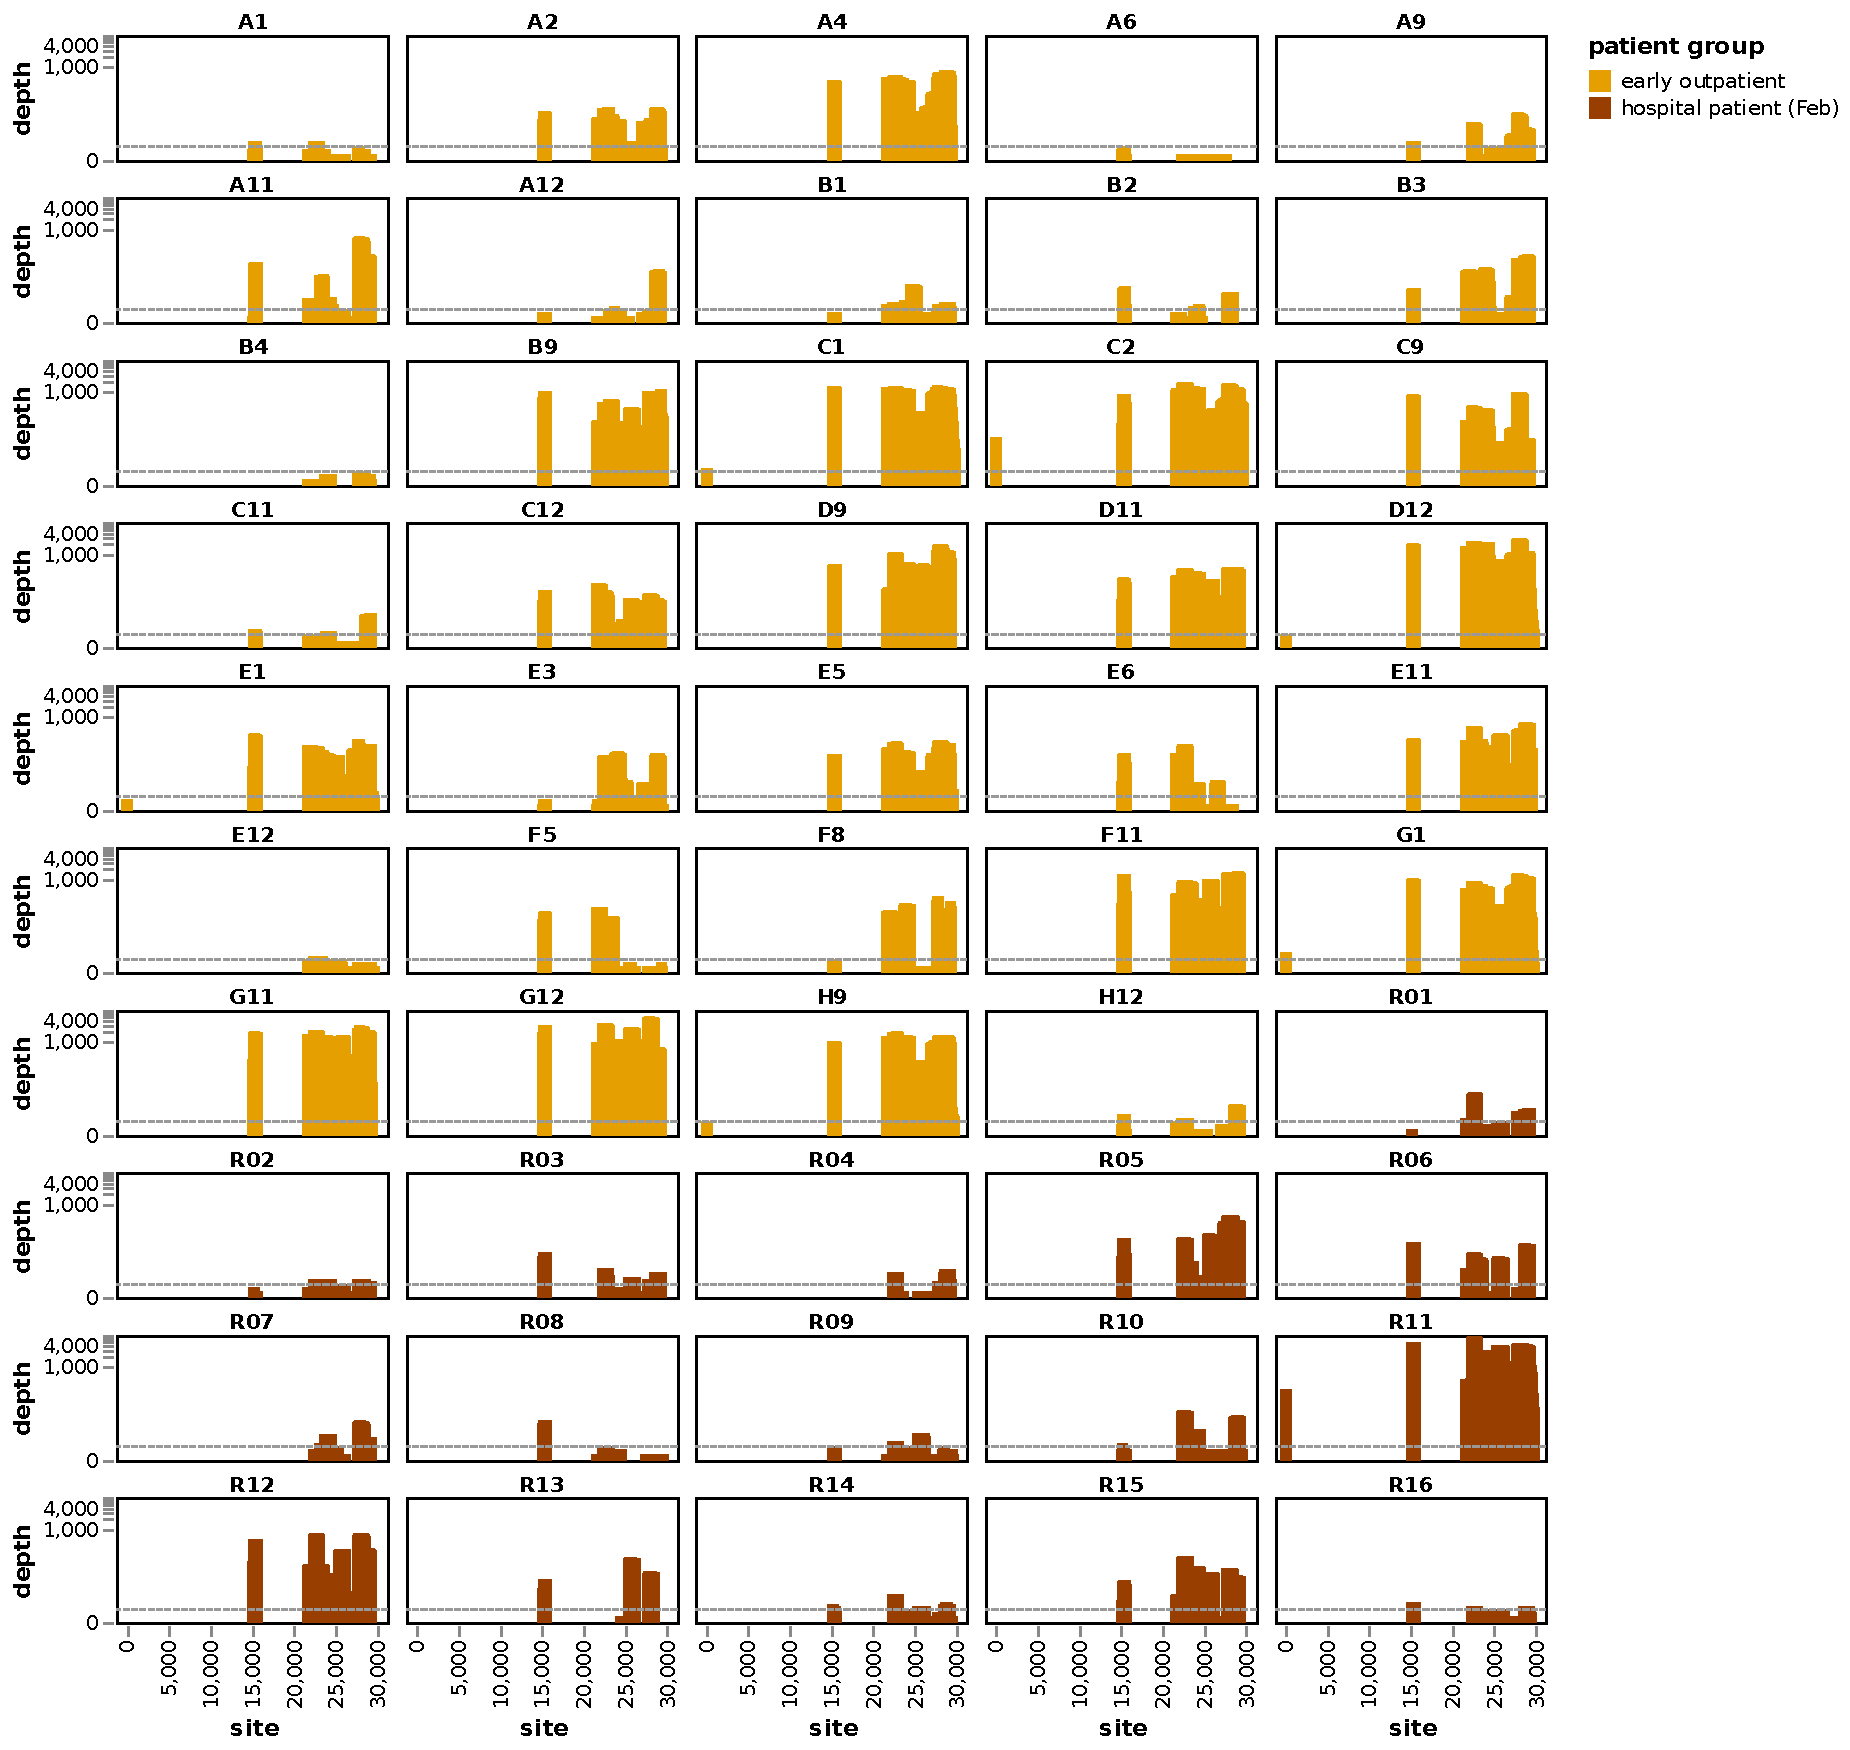
\includegraphics[width=\linewidth]{figures/coverage_all.pdf}
\caption{A version of Figure~\ref{fig:coverage} that shows coverage over the full length of the SARS-CoV-2 genome.
An interactive version of this plot is at {\color{red} add link}.
}
\label{suppfig:coverage_all}
\end{figure}

\begin{figure}[h!]
{\bf \LARGE A} \\
\centerline{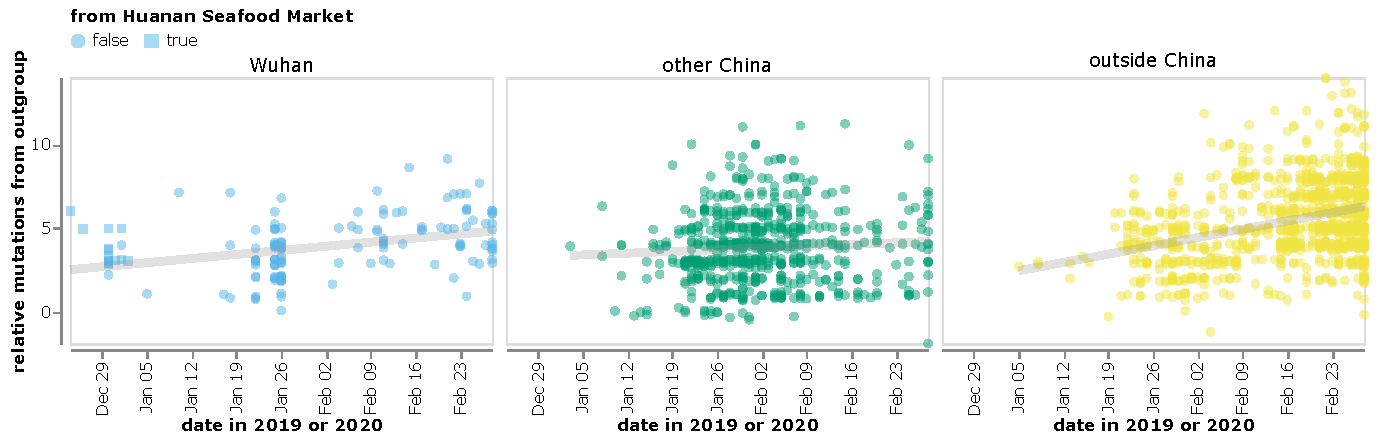
\includegraphics[width=\linewidth]{figures/deltadist_RpYN06.pdf}}
{\bf \LARGE B} \\
\centerline{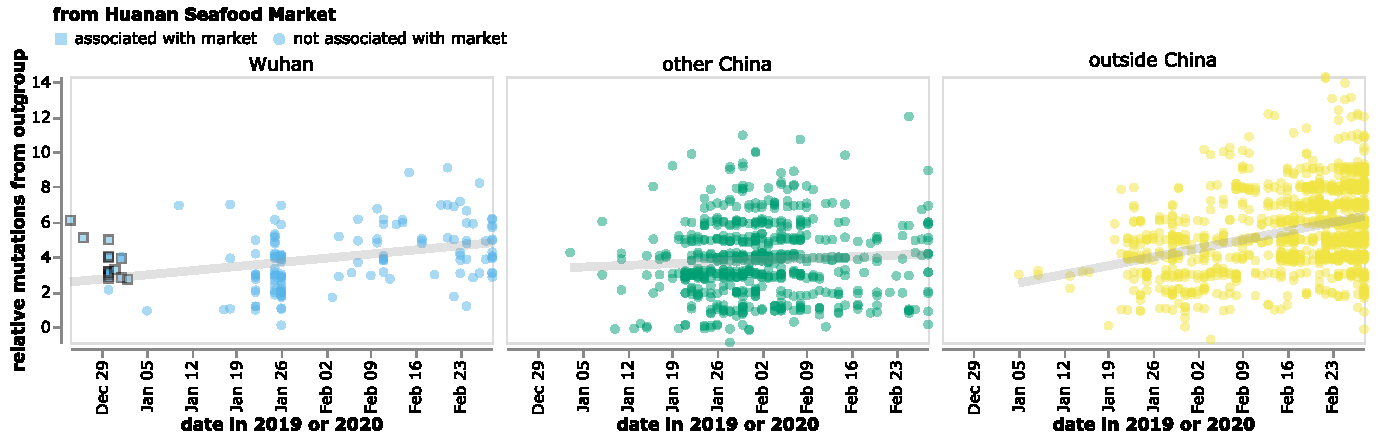
\includegraphics[width=\linewidth]{figures/deltadist_RmYN02.pdf}}
\caption{Versions of Figure~\ref{fig:deltadist_RaTG13} but calculating the relative mutational distances using an outgroup of (A) RpYN06 or (B) RmYN02.
}
\label{suppfig:deltadist_RpYN06_RmYN02}
\end{figure}

 \begin{figure}[h!]
 {\bf \LARGE A} \\
 \centerline{
 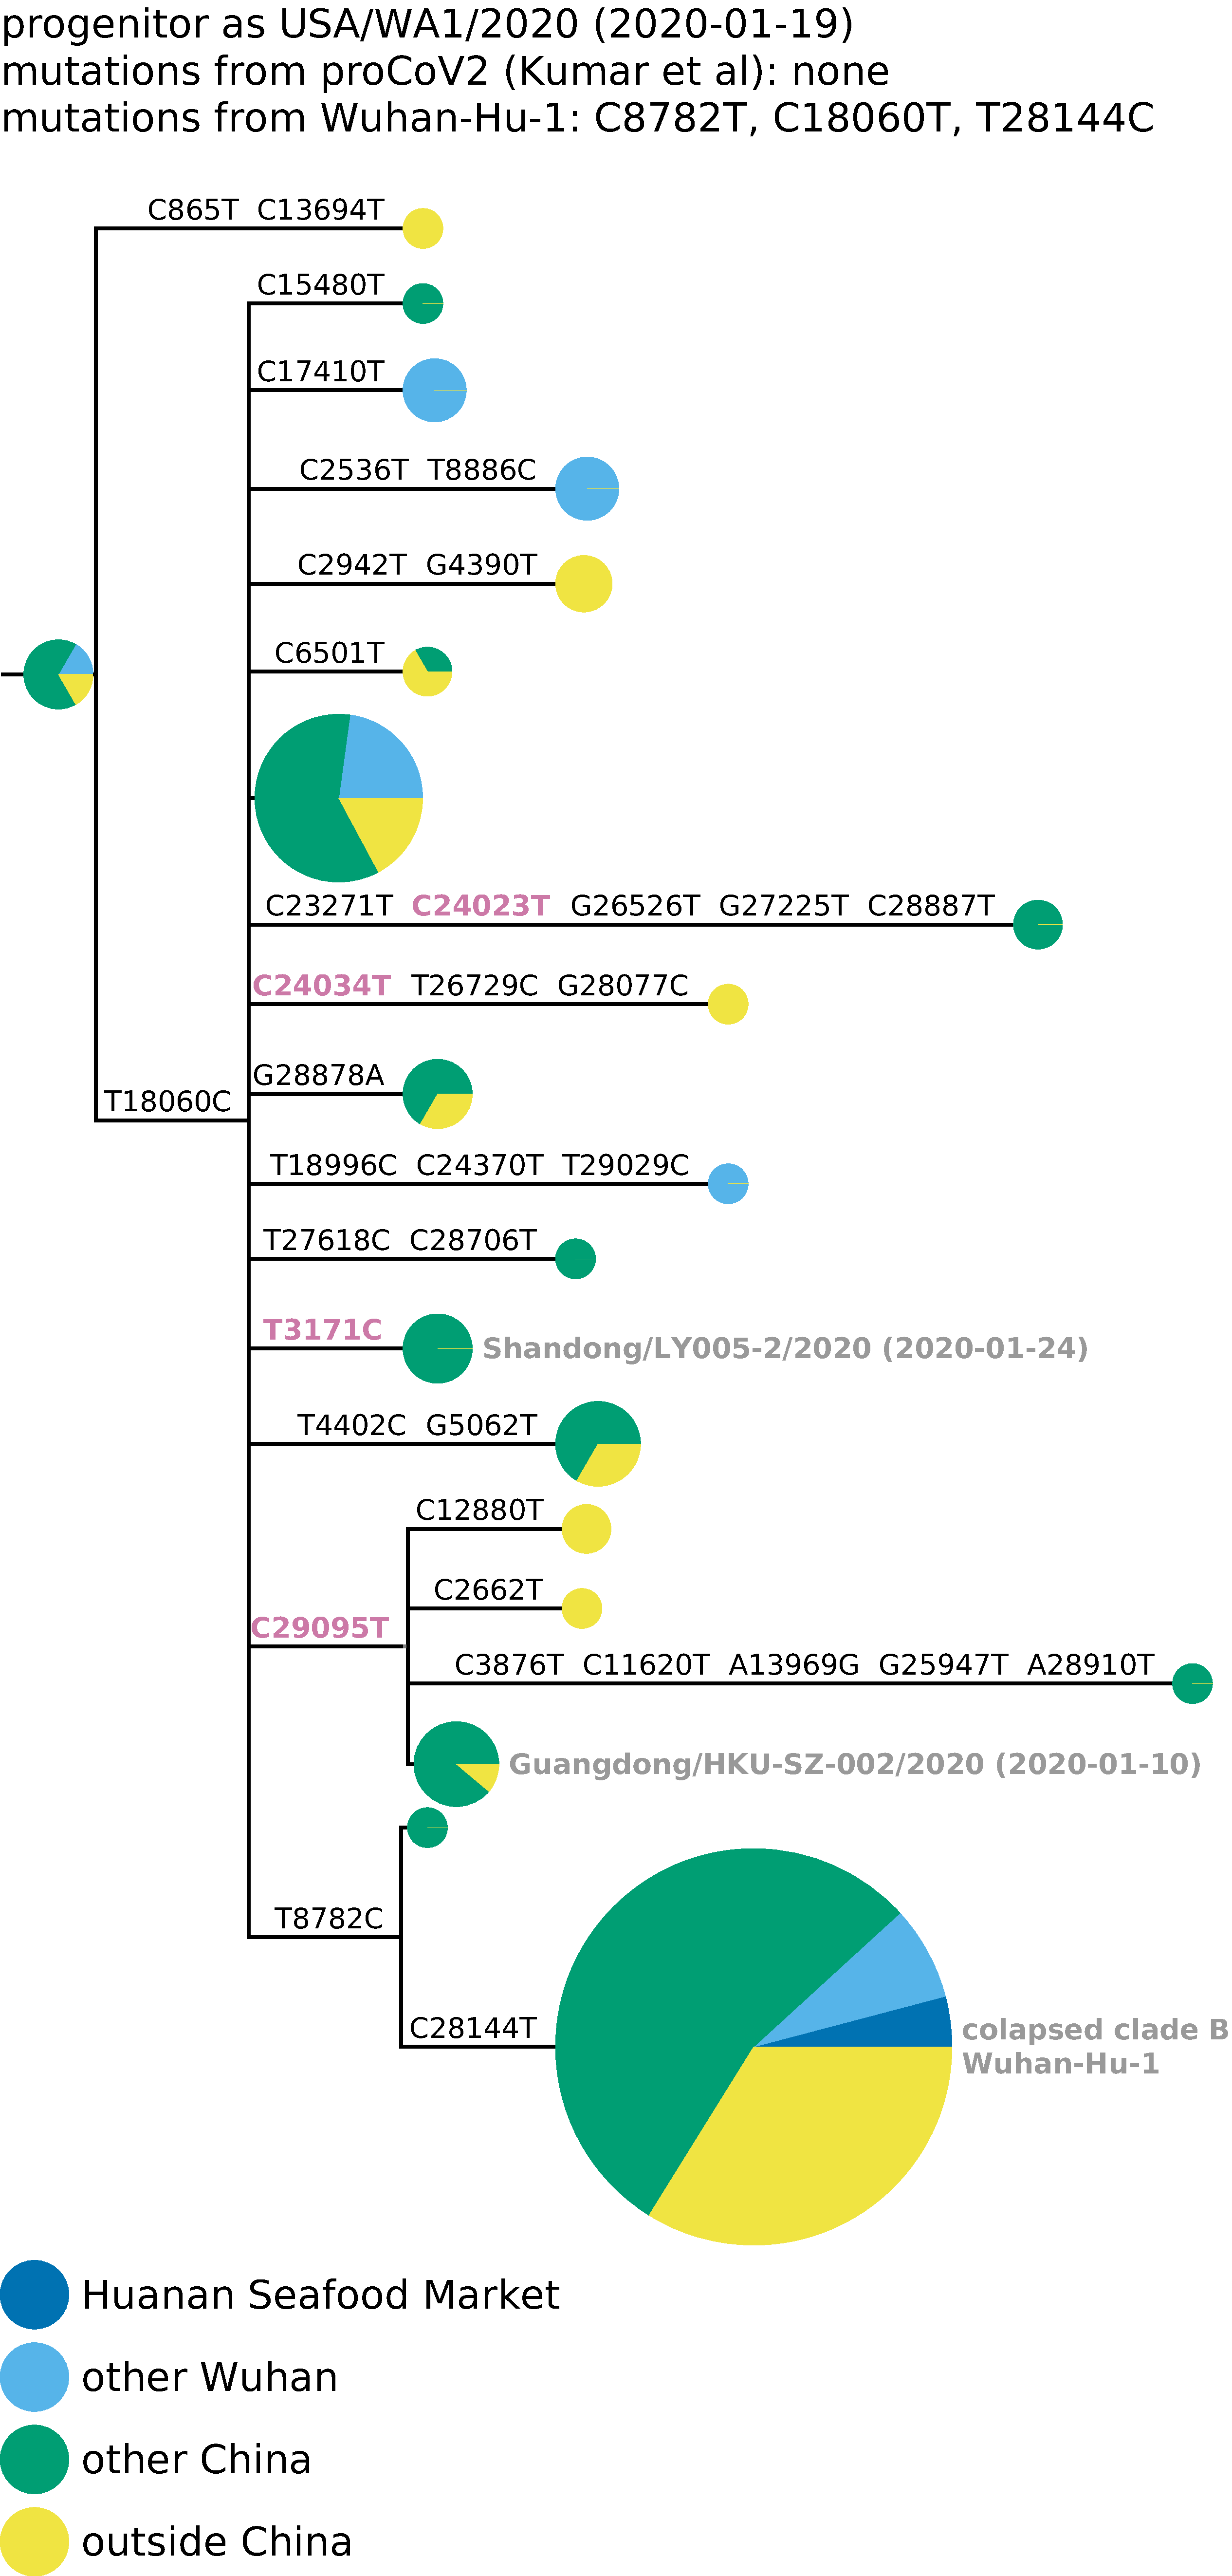
\includegraphics[width=0.3\linewidth, valign=t, clip=true, trim=0in 4.4in 0in 0in]{figures/tree_images/hCoV-19-USA-WA1-2020_RpYN06_without_deleted_seqs.pdf}
 \hspace{0.04\linewidth}
 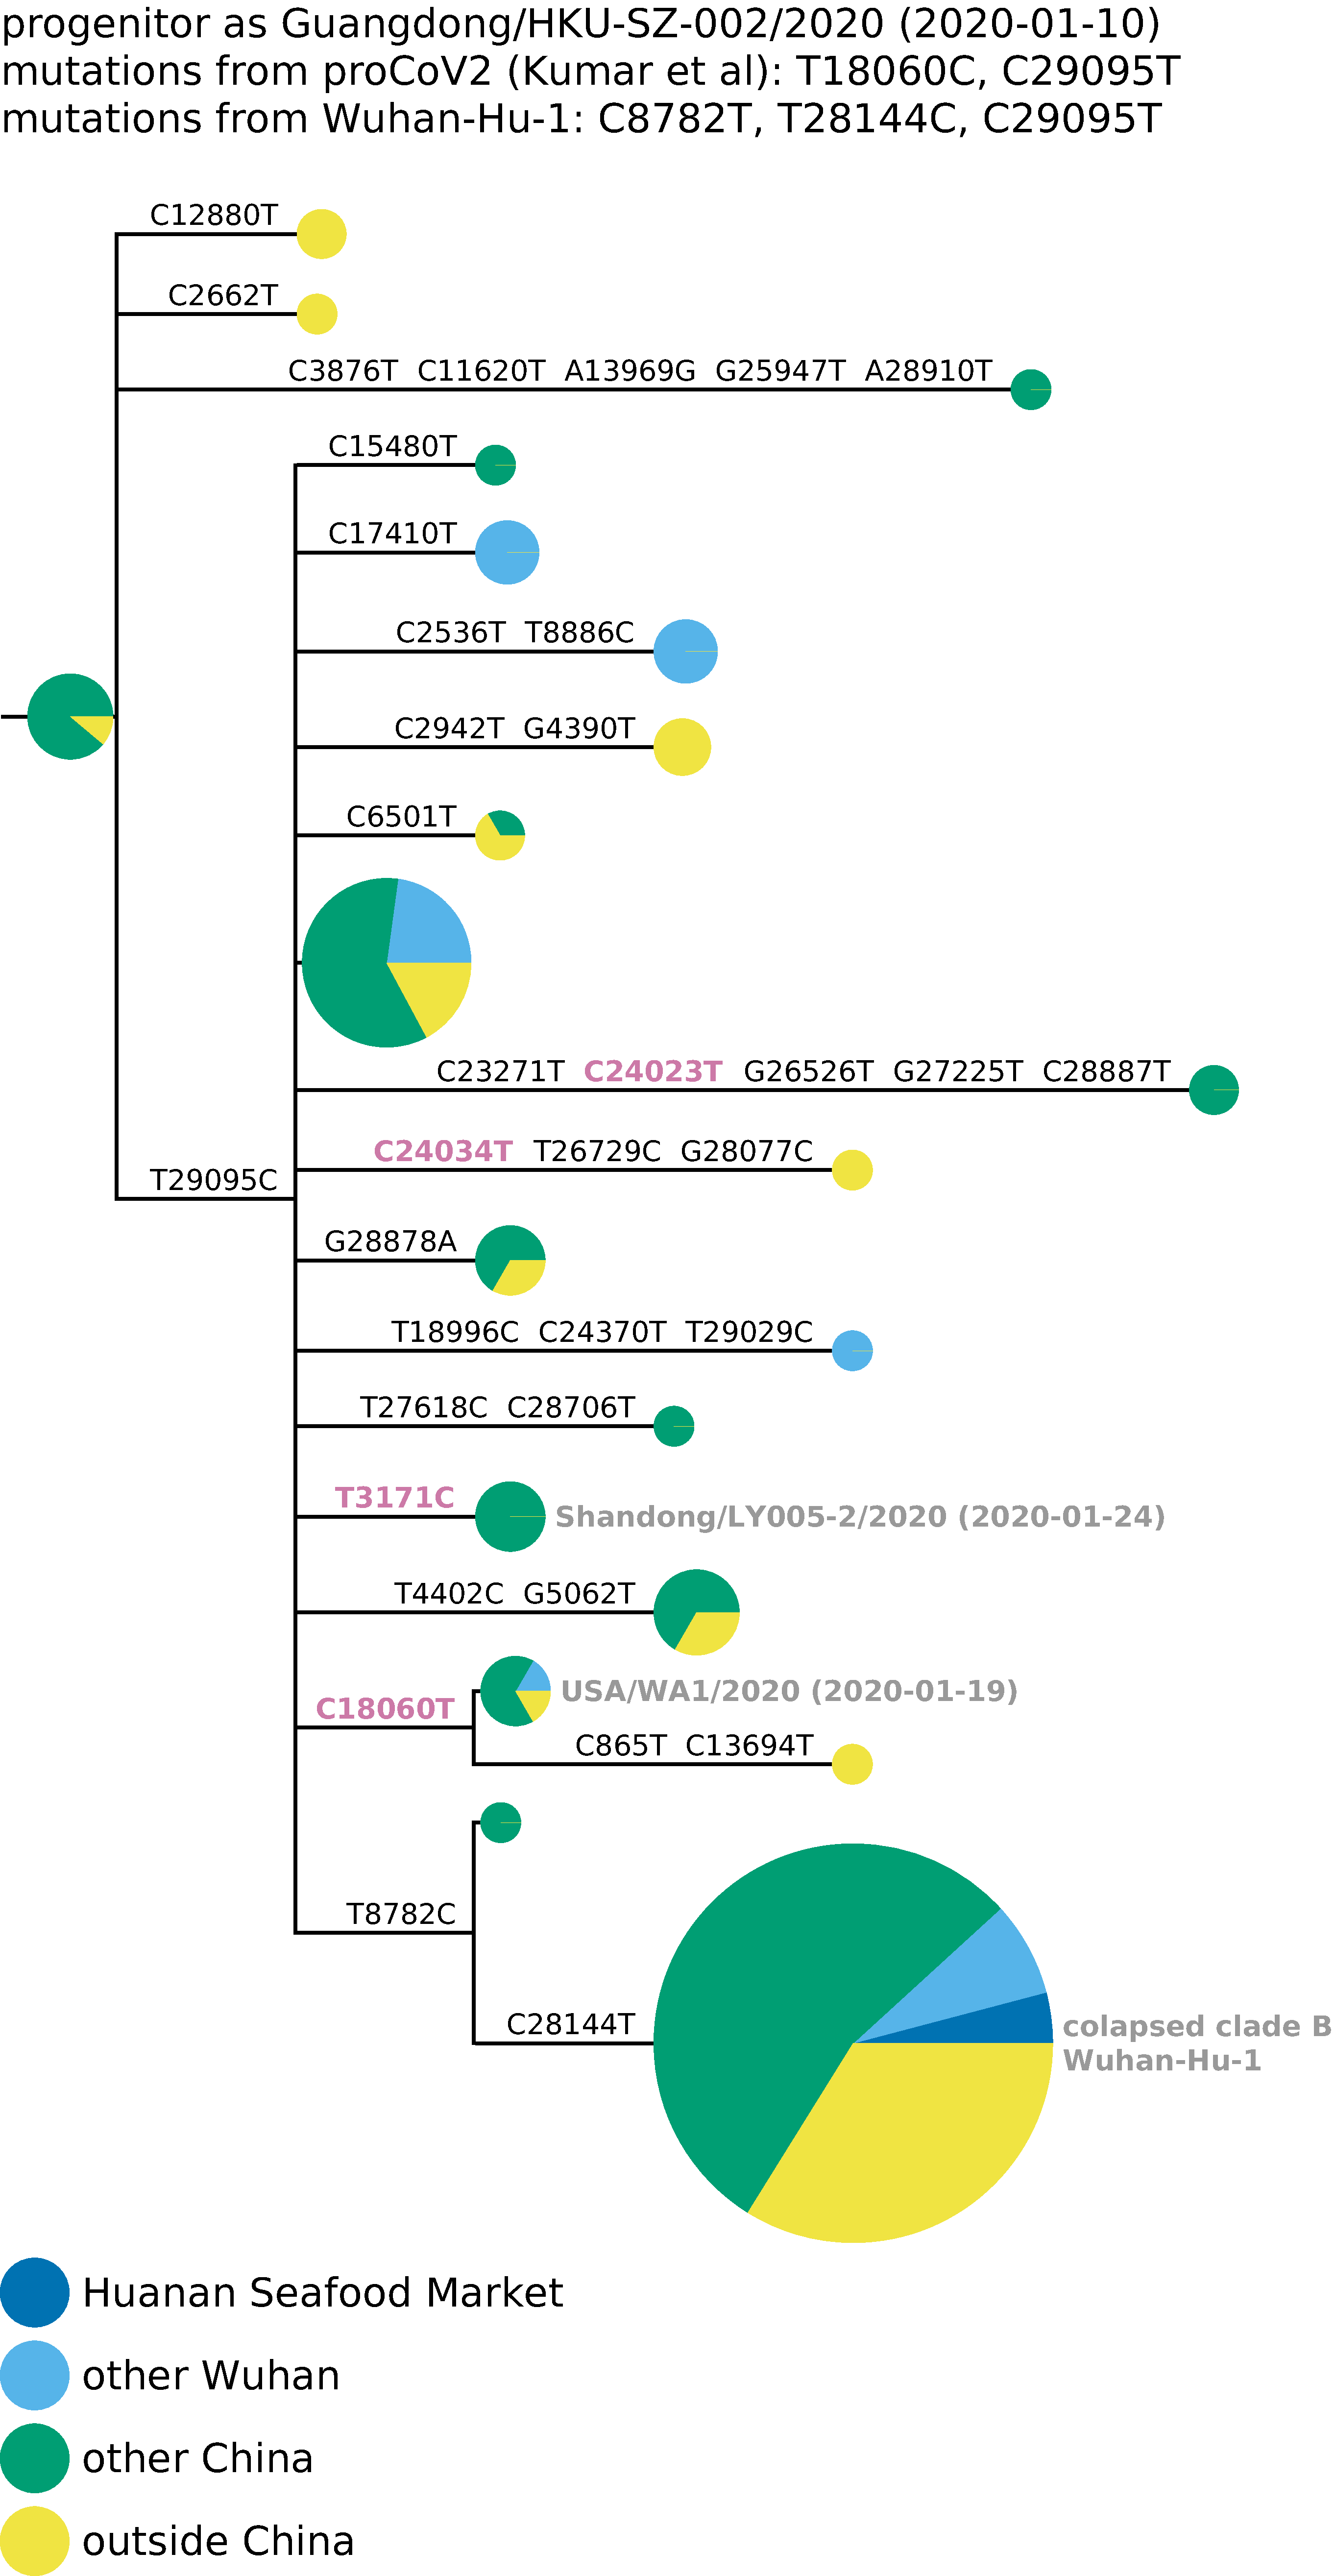
\includegraphics[width=0.32\linewidth, valign=t, clip=true]{figures/tree_images/hCoV-19-Guangdong-HKU-SZ-002-2020_RpYN06_without_deleted_seqs.pdf}
  \hspace{0.04\linewidth}
 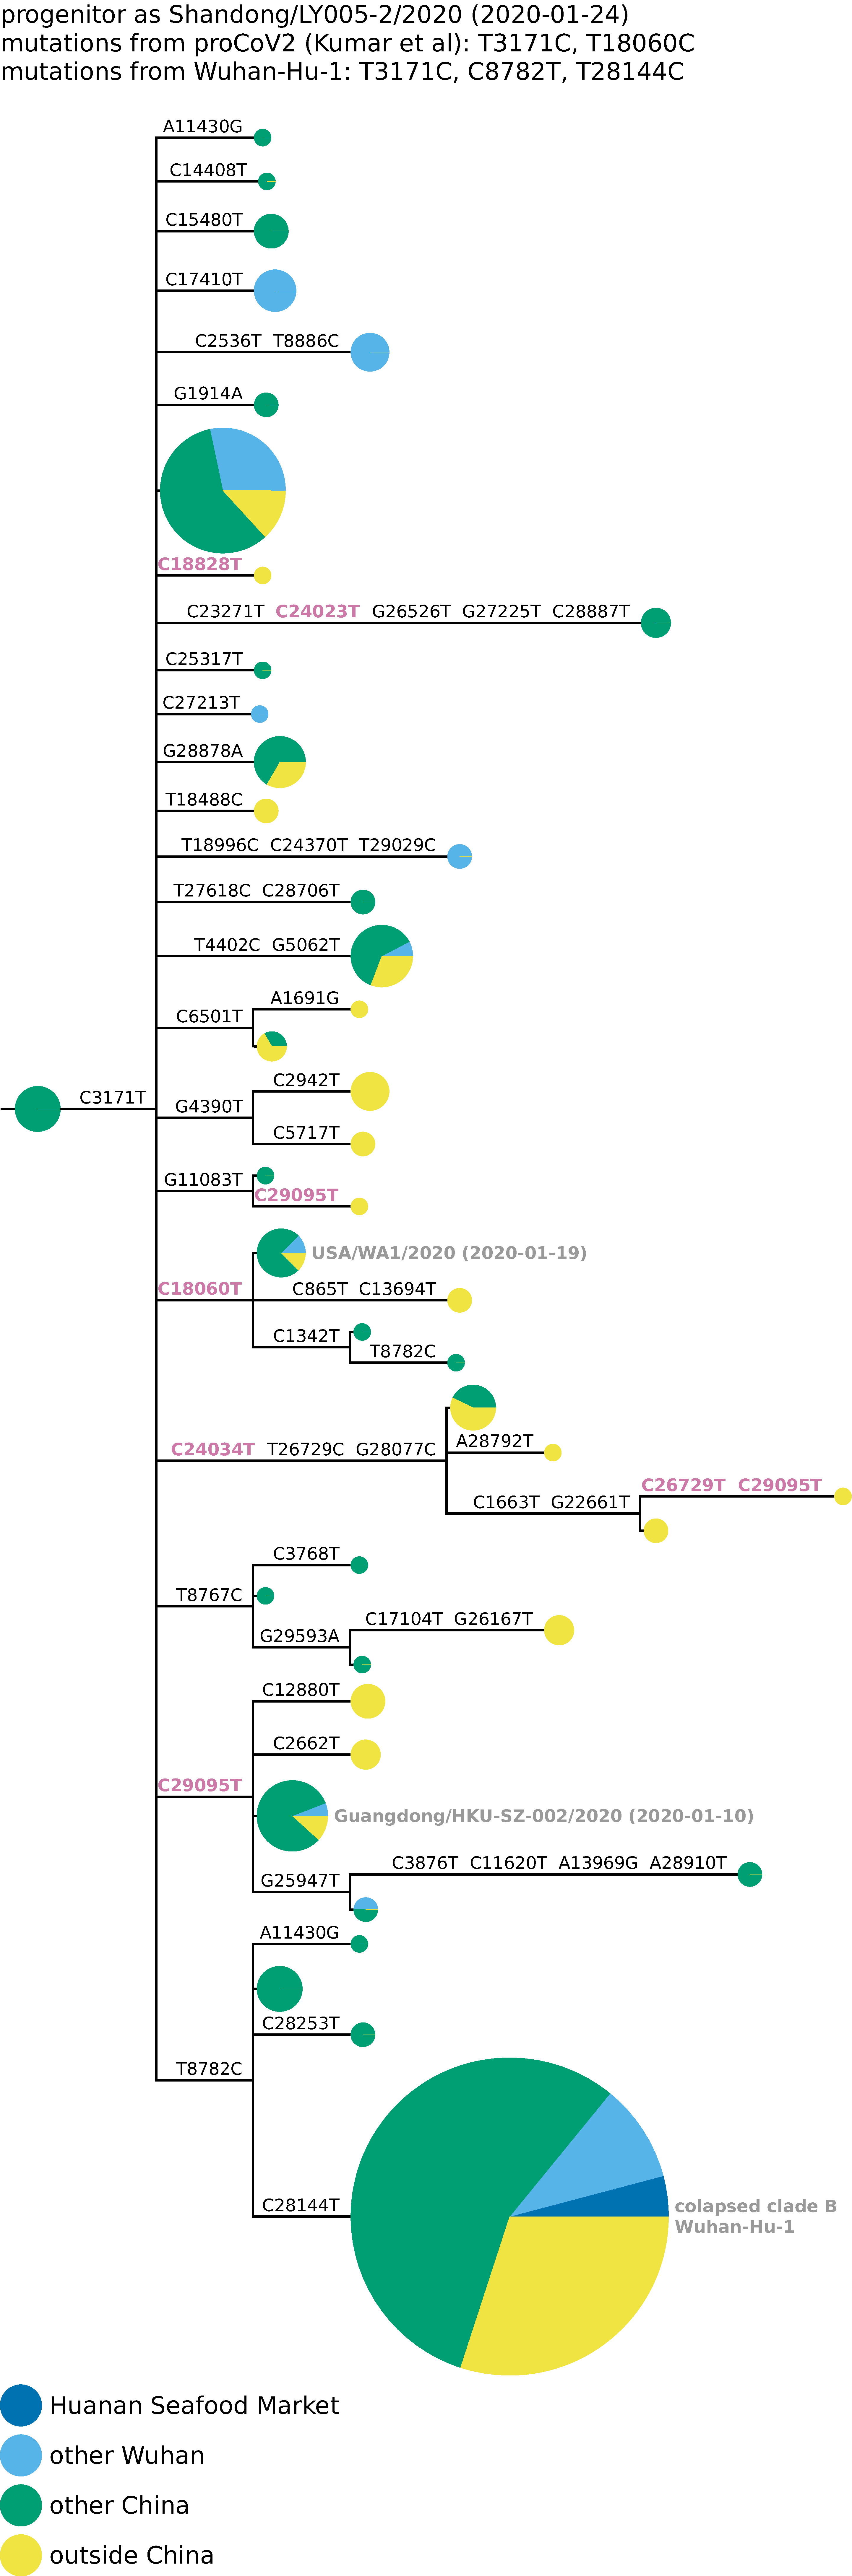
\includegraphics[width=0.3\linewidth, valign=t, clip=true, trim=0in 4.4in 0in 0in]{figures/tree_images/hCoV-19-Shandong-LY005-2-2020_RpYN06_without_deleted_seqs.pdf}
 }
 \\
  {\bf \LARGE B} \\
 \centerline{
 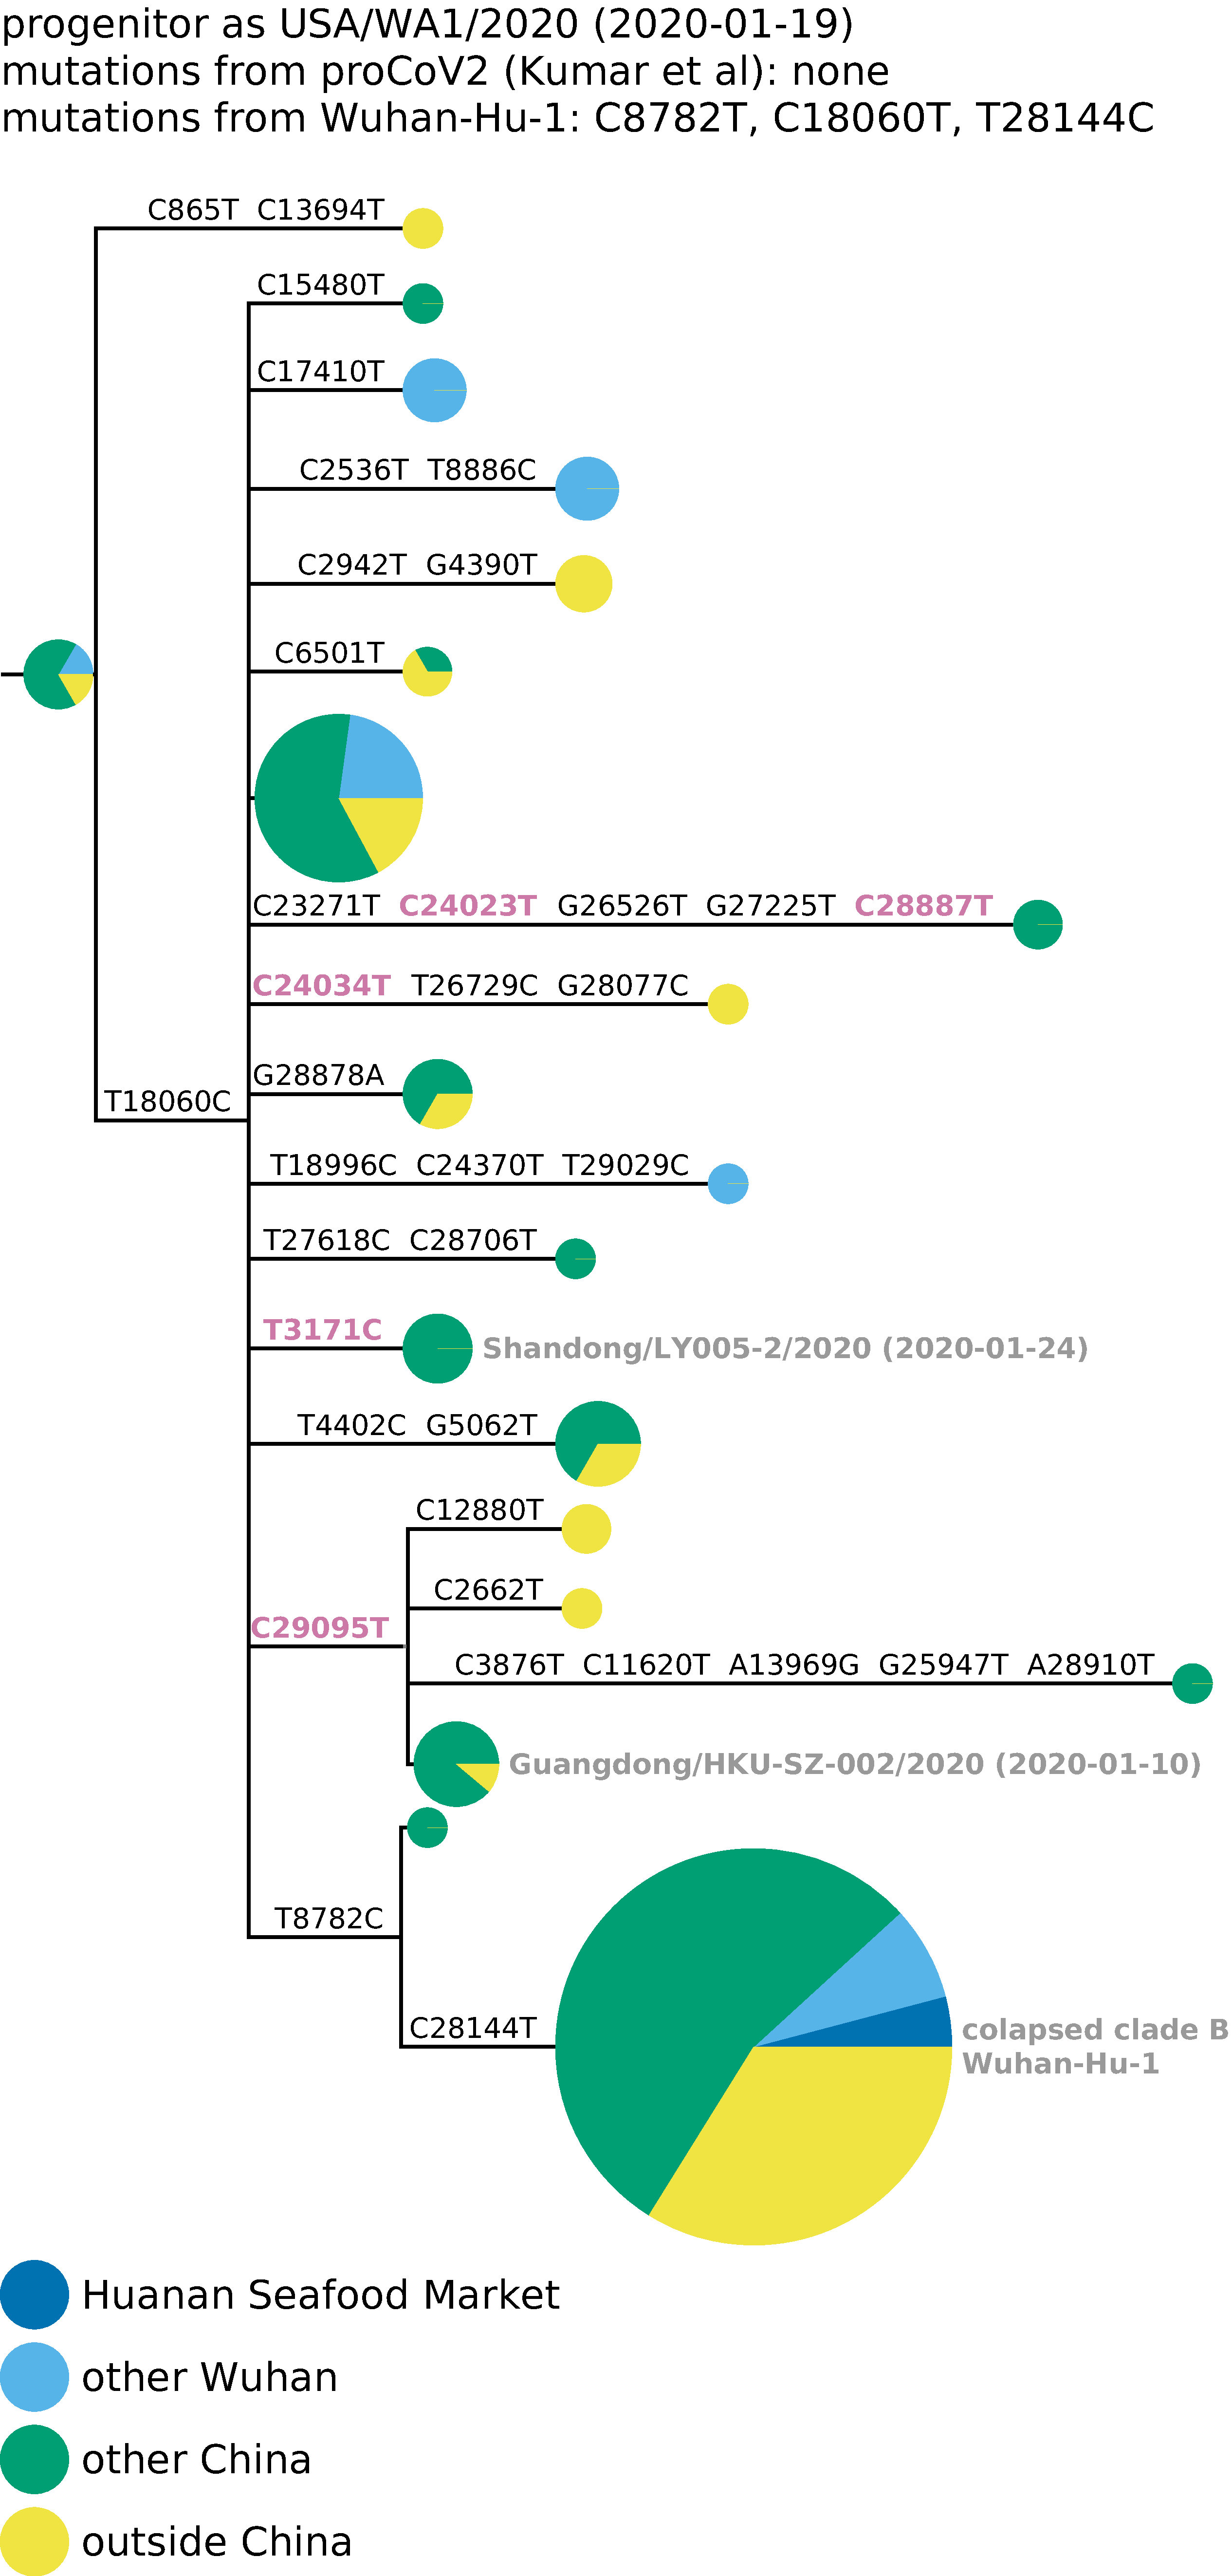
\includegraphics[width=0.3\linewidth, valign=t, clip=true, trim=0in 4.4in 0in 0in]{figures/tree_images/hCoV-19-USA-WA1-2020_RmYN02_without_deleted_seqs.pdf}
 \hspace{0.04\linewidth}
 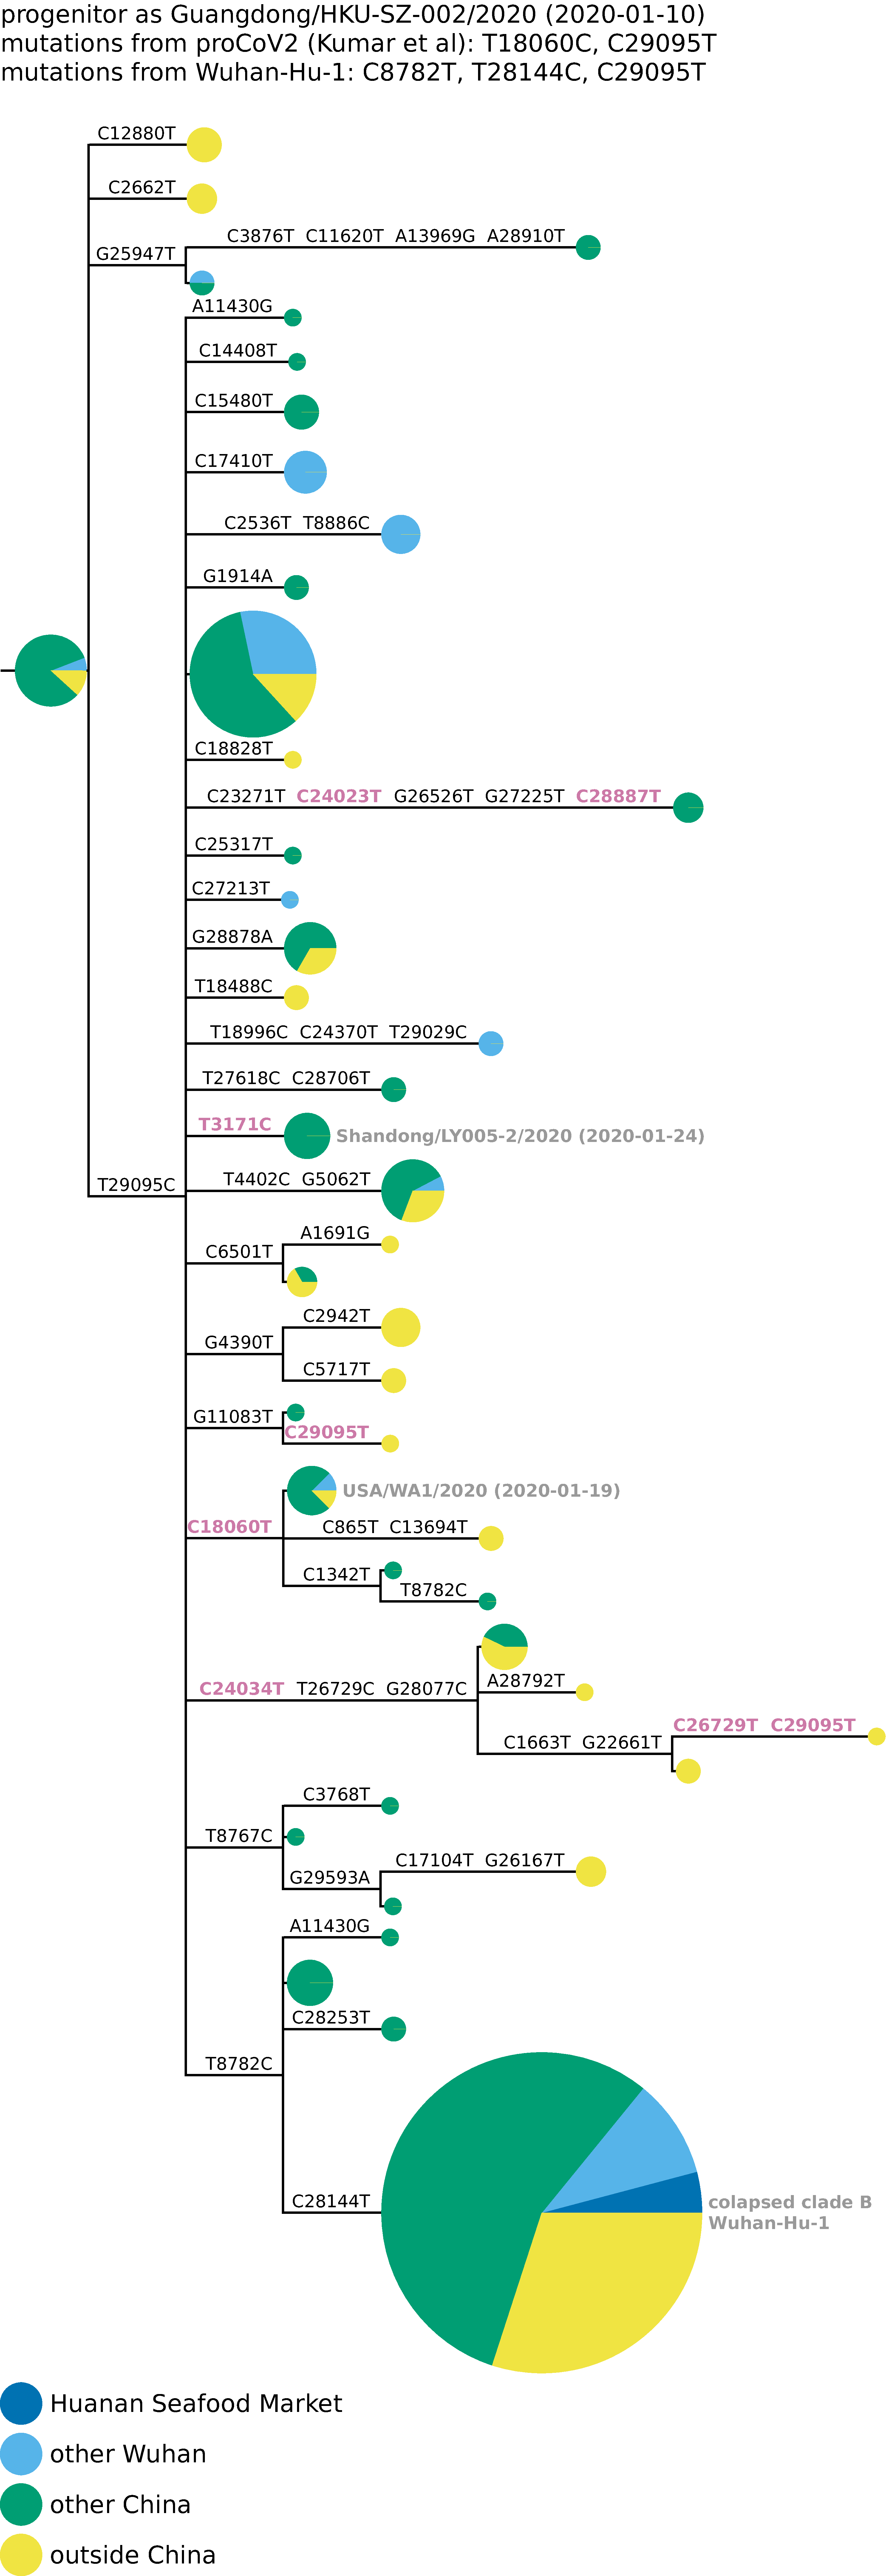
\includegraphics[width=0.32\linewidth, valign=t, clip=true, trim=0in 4.4in 0in 0in]{figures/tree_images/hCoV-19-Guangdong-HKU-SZ-002-2020_RmYN02_without_deleted_seqs.pdf}
  \hspace{0.04\linewidth}
 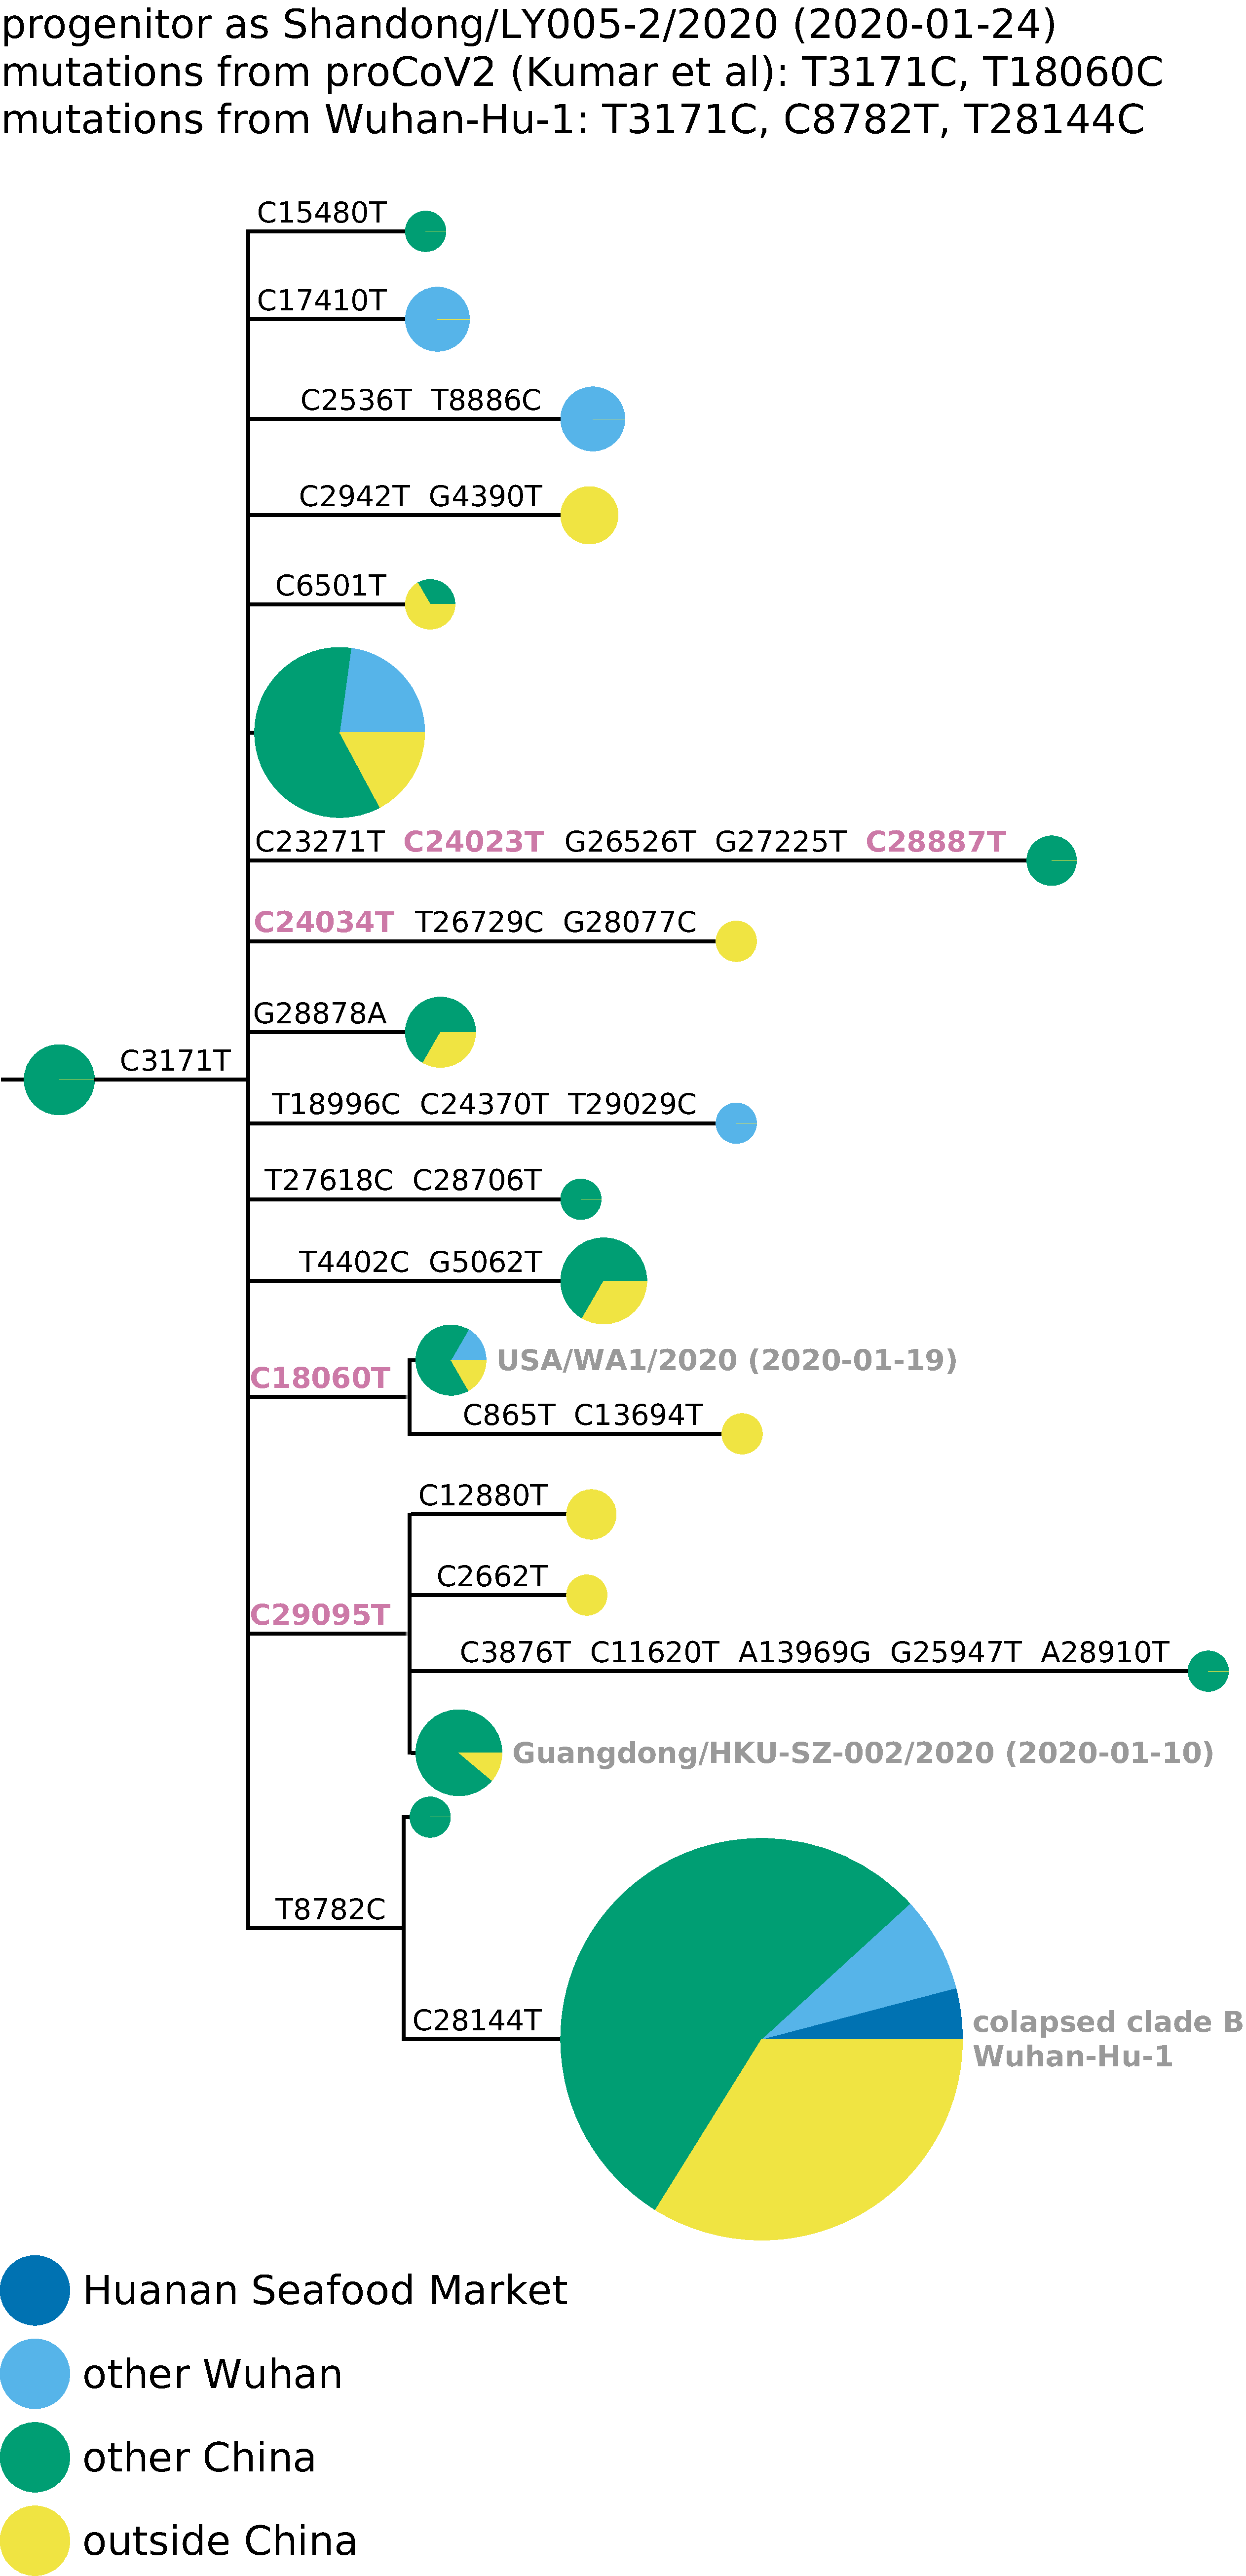
\includegraphics[width=0.3\linewidth, valign=t, clip=true, trim=0in 4.4in 0in 0in]{figures/tree_images/hCoV-19-Shandong-LY005-2-2020_RmYN02_without_deleted_seqs.pdf}
 }
 \caption{
 A version of Figure~\ref{fig:tree_RaTG13} but rooting using an outgroup of (A) RpYN06 or (B) RmYN02 outgroups.
 The tree topologies are identical to those obtained using RaTG13 in Figure~\ref{fig:tree_RaTG13}, with the only differences being a few minor changes in which mutations on branches are towards the outgroup (purple mutation labels).
\label{suppfig:tree_RpYN06_RmYN02}
 }
 \end{figure}



\end{document}
